\documentclass[10pt,aspectratio=169,mathserif]{beamer}
\usepackage{jsu}
\usepackage[UTF8]{ctex}
\usepackage{xeCJK}
\usepackage{amsmath,amsfonts,amssymb,bm}
\usepackage{color}
\usepackage{ulem}
\usepackage{graphicx,hyperref,url}
\usepackage{listings}
\usepackage{tikz}
\usetikzlibrary{shapes.geometric, arrows, positioning}

\lstset{
    language=C, % 设置语言为C
    backgroundcolor=\color{white},
    basicstyle=\ttfamily\color{black}\tiny,
    keywordstyle=\color{blue},
    commentstyle=\color{green!60!black},
    stringstyle=\color{purple},
    numbers=left,
    numberstyle=\tiny\color{gray},
    frame=single,
    breaklines=true,
    tabsize=4,
    columns=fullflexible,
}

\beamertemplateballitem

\title{UniTrack：GPS+IMU融合的跨场景全维度\\运动轨迹与状态监测系统}

\author[徐奕博]{
    徐奕博\ 通信2402\\
    学号：3240601042\\
  {\small \url{https://github.com/XCMB-haochi}}}

\date{2025年11月}

\begin{document}

%% 封面
\begin{frame}
    \titlepage
\end{frame}

%% 目录
\begin{frame}
    \frametitle{目录}
    \tableofcontents
\end{frame}

%% 第一部分：项目概述
\section{项目概述}

\begin{frame}{项目背景与目标}
    \begin{columns}
    \column{0.5\textwidth}
    \textbf{设计目标：}
    \begin{itemize}
        \item 实时采集GPS定位数据
        \item 实时采集IMU姿态数据
        \item SD卡持久化存储（FATFS）
        \item LCD本地实时显示（LVGL）
        \item Web端轨迹可视化分析
    \end{itemize}

    \column{0.5\textwidth}
    \textbf{应用场景：}
    \begin{itemize}
        \item 运动轨迹记录（骑行、跑步）
        \item 车辆行驶记录（黑匣子）
        \item 无人机飞行监测
        \item 设备运动状态分析
        \item 数据科学研究
    \end{itemize}
    \end{columns}
\end{frame}

\begin{frame}{系统架构}
\begin{center}
\begin{tikzpicture}[scale=0.85, every node/.style={scale=0.85}]
    % 定义样式
    \tikzstyle{mcu} = [rectangle, draw, fill=blue!20, text width=5cm, text centered, minimum height=1cm, font=\bfseries]
    \tikzstyle{sensor} = [rectangle, draw, fill=green!20, text width=1.6cm, text centered, minimum height=0.8cm]
    \tikzstyle{ui} = [rectangle, draw, fill=orange!20, text width=5cm, text centered, minimum height=0.8cm]
    \tikzstyle{web} = [rectangle, draw, fill=purple!20, text width=5cm, text centered, minimum height=0.8cm]
    \tikzstyle{arrow} = [thick,->,>=stealth]

    % 节点
    \node (mcu) [mcu] at (0,0) {STM32F407ZGT6\\168MHz | 1MB Flash | 192KB RAM};

    \node (gps) [sensor] at (-2.5,-2) {GPS模块\\ATK1218-BD};
    \node (imu) [sensor] at (0,-2) {IMU模块\\MPU6050};
    \node (sd) [sensor] at (2.5,-2) {SD卡\\FATFS};

    \node (lcd) [ui] at (0,-3.5) {LCD显示屏\\LVGL 5.3 图形库};

    \node (web) [web] at (0,-5) {Web可视化系统\\Leaflet.js + Chart.js};

    % 连接线
    \draw [arrow] (gps) -- (mcu) node[midway,left,font=\tiny] {UART1};
    \draw [arrow] (imu) -- (mcu) node[midway,left,font=\tiny] {I2C1};
    \draw [arrow] (sd) -- (mcu) node[midway,right,font=\tiny] {SDIO};
    \draw [arrow] (mcu) -- (lcd) node[midway,right,font=\tiny] {FSMC};
    \draw [arrow] (sd) -- (web) node[midway,right,font=\tiny] {CSV};
\end{tikzpicture}
\end{center}
\end{frame}

\begin{frame}{硬件配置清单}
\begin{table}
\centering
\small
\begin{tabular}{|c|c|c|c|}
\hline
\textbf{模块} & \textbf{型号} & \textbf{接口} & \textbf{功能} \\
\hline
主控MCU & STM32F407ZGT6 & - & 168MHz, 1MB Flash, 192KB RAM \\
\hline
GPS模块 & ATK1218-BD & UART1 (115200) & GPS/北斗双模定位 \\
\hline
IMU传感器 & MPU6050 & I2C1 (0x68) & 6轴姿态+DMP硬件解算 \\
\hline
存储器 & Micro SD卡 & SDIO (25MHz) & FATFS文件系统 \\
\hline
显示屏 & TFT LCD & FSMC & 320×240 LVGL界面 \\
\hline
\end{tabular}
\end{table}
\end{frame}

%% 第二部分：关键技术
\section{关键技术实现}

\begin{frame}{GPS数据采集}
    \begin{columns}
    \column{0.45\textwidth}
    \textbf{技术要点：}
    \begin{itemize}
        \item NMEA-0183协议解析
        \item \$GPRMC：推荐最小定位信息
        \item \$GPGGA：定位质量数据
        \item 波特率：115200
        \item 经纬度格式转换
    \end{itemize}

    \vspace{0.1cm}
    \textbf{{\color{red}调试难点：}}
    \begin{itemize}
        \item {\color{red}跳线帽连接错误}
        \item 模块型号识别问题
        \item 波特率配置
    \end{itemize}

    \column{0.55\textwidth}
    \begin{center}
    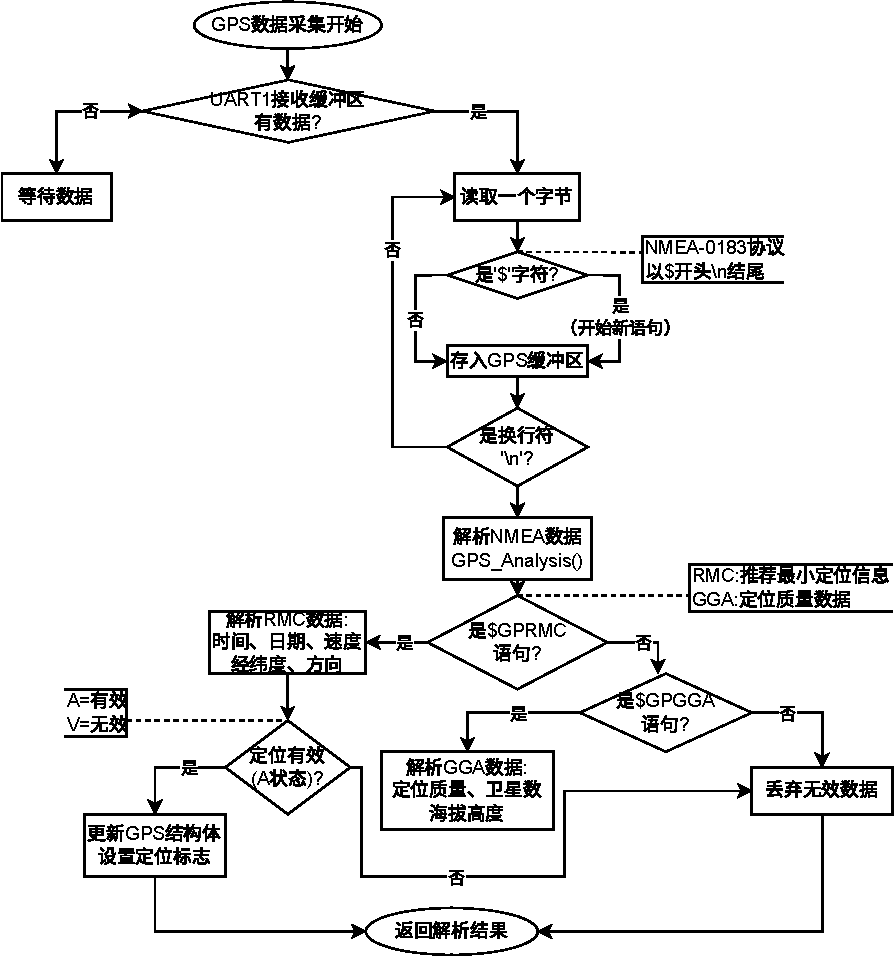
\includegraphics[height=0.75\textheight]{flowcharts/gps_acquisition.pdf}
    \end{center}
    \end{columns}
\end{frame}

\begin{frame}{GPS模块调试过程}
    \begin{block}{问题现象}
    LCD只显示部分内容，GPS数据一直显示"NEO-6M Setting..."，无法获取定位数据
    \end{block}

    \begin{block}{{\color{red}问题根源}}
    \begin{enumerate}
        \item {\color{red}跳线帽连接错误：}P2端子未正确短接PB10(TX)-GBC\_R和PB11(RX)-GBC\_TX
        \item {\color{red}模块识别错误：}例程基于NEO-6M，实际使用ATK1218-BD
        \item 波特率设置：需要115200而非9600
    \end{enumerate}
    \end{block}

    \begin{block}{{\color{green!60!black}解决方案}}
    \begin{itemize}
        \item 重新连接跳线帽（参考ATK-MO1218使用说明P2）
        \item 切换到正确的ATK1218-BD例程
        \item 设置波特率115200，按下KEY0启用"NMEA Data Upload:ON"
        \item 成功在串口助手和GNSS\_Viewer接收到定位数据
    \end{itemize}
    \end{block}
\end{frame}

\begin{frame}{IMU姿态解算}
    \begin{columns}
    \column{0.45\textwidth}
    \textbf{DMP硬件解算：}
    \begin{itemize}
        \item Digital Motion Processor
        \item 四元数→欧拉角转换
        \item Pitch：俯仰角 (±90°)
        \item Roll：翻滚角 (±180°)
        \item Yaw：航向角 (0\textasciitilde 360°)
        \item 实时温度监测
    \end{itemize}

    \vspace{0.1cm}
    \textbf{I2C通信：}
    \begin{itemize}
        \item 地址：0x68 (AD0=0)
        \item FIFO深度：1024字节
        \item 采样率：100Hz
    \end{itemize}

    \column{0.55\textwidth}
    \begin{center}
    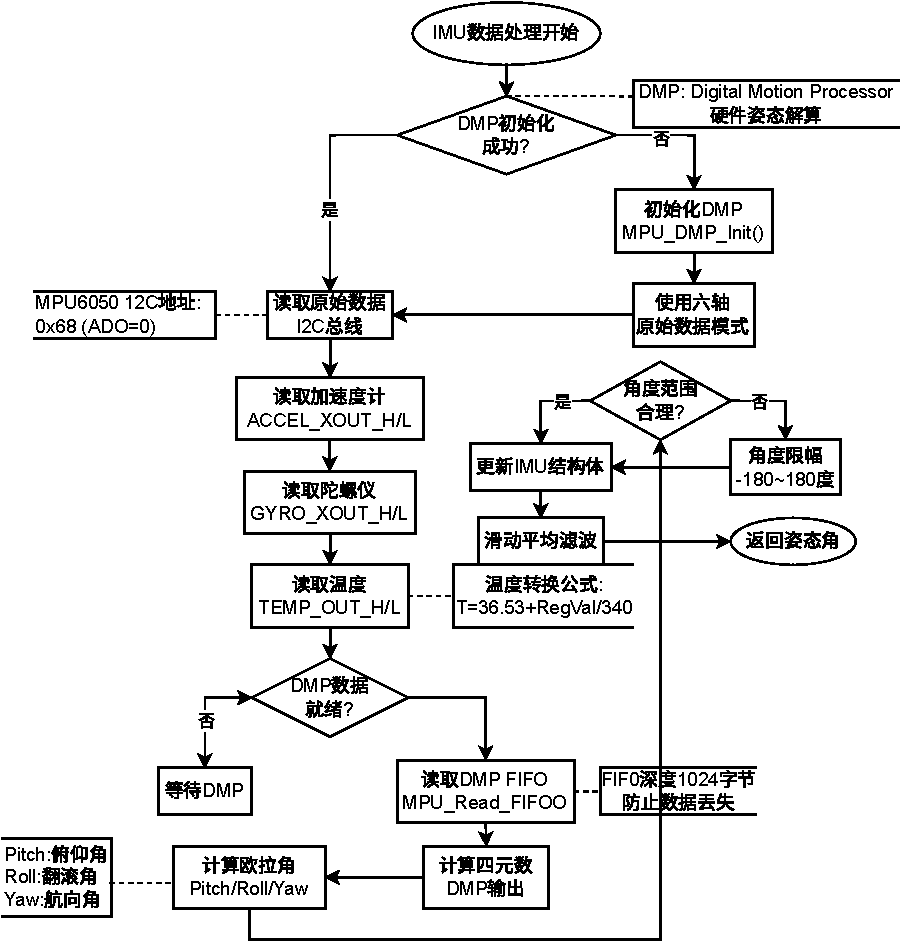
\includegraphics[height=0.75\textheight]{flowcharts/imu_processing.pdf}
    \end{center}
    \end{columns}
\end{frame}

\begin{frame}{SD卡文件系统}
    \begin{columns}
    \column{0.5\textwidth}
    \textbf{{\color{red}关键问题：内存不足}}
    \begin{block}{L6406E错误 (61条)}
    \begin{itemize}
        \item {\color{red}初始malloc：100KB → 编译失败}
        \item {\color{red}IRAM1错误配置：192KB}
        \item {\color{red}勾选IRAM2 → L6971E冲突}
    \end{itemize}
    \end{block}

    \begin{block}{{\color{green!60!black}最终方案}}
    \begin{itemize}
        \item IRAM1：128KB（正确值）
        \item malloc：40KB（降低需求）
        \item 使用CCM内存管理
        \item 补充DMA/SDIO/SPI外设库
    \end{itemize}
    \end{block}

    \column{0.5\textwidth}
    \textbf{文件管理策略：}
    \begin{itemize}
        \item FA\_CREATE\_NEW（防覆盖）
        \item 自动索引：data\_000.csv
        \item 断电保护机制
        \item 定期f\_sync()同步
    \end{itemize}

    \vspace{0.1cm}
    \textbf{CSV数据格式：}\\
    {\tiny\ttfamily
    Time,Lat,LatDir,Lon,\\
    LonDir,Speed,Alt,Sats,\\
    Pitch,Roll,Yaw,Temp
    }

    \vspace{0.2cm}
    \begin{center}
    \small
    单条80字节 | 10Hz采样\\
    1小时$\approx$2.8MB | 8GB卡>2000小时
    \end{center}
    \end{columns}
\end{frame}

\begin{frame}{LVGL图形界面}
    \begin{columns}
    \column{0.4\textwidth}
    \textbf{4-Tab页面设计：}
    \begin{itemize}
        \item \textbf{Home：}系统状态总览
        \item \textbf{GPS：}定位信息实时显示
        \item \textbf{IMU：}姿态角度可视化
        \item \textbf{Files：}文件管理器
    \end{itemize}

    \vspace{0.3cm}
    \textbf{交互功能：}
    \begin{itemize}
        \item Start/Stop Log切换按钮
        \item Dark/Light模式切换
        \item 文件浏览与删除
        \item Refresh刷新列表
    \end{itemize}

    \column{0.6\textwidth}
    \begin{center}
    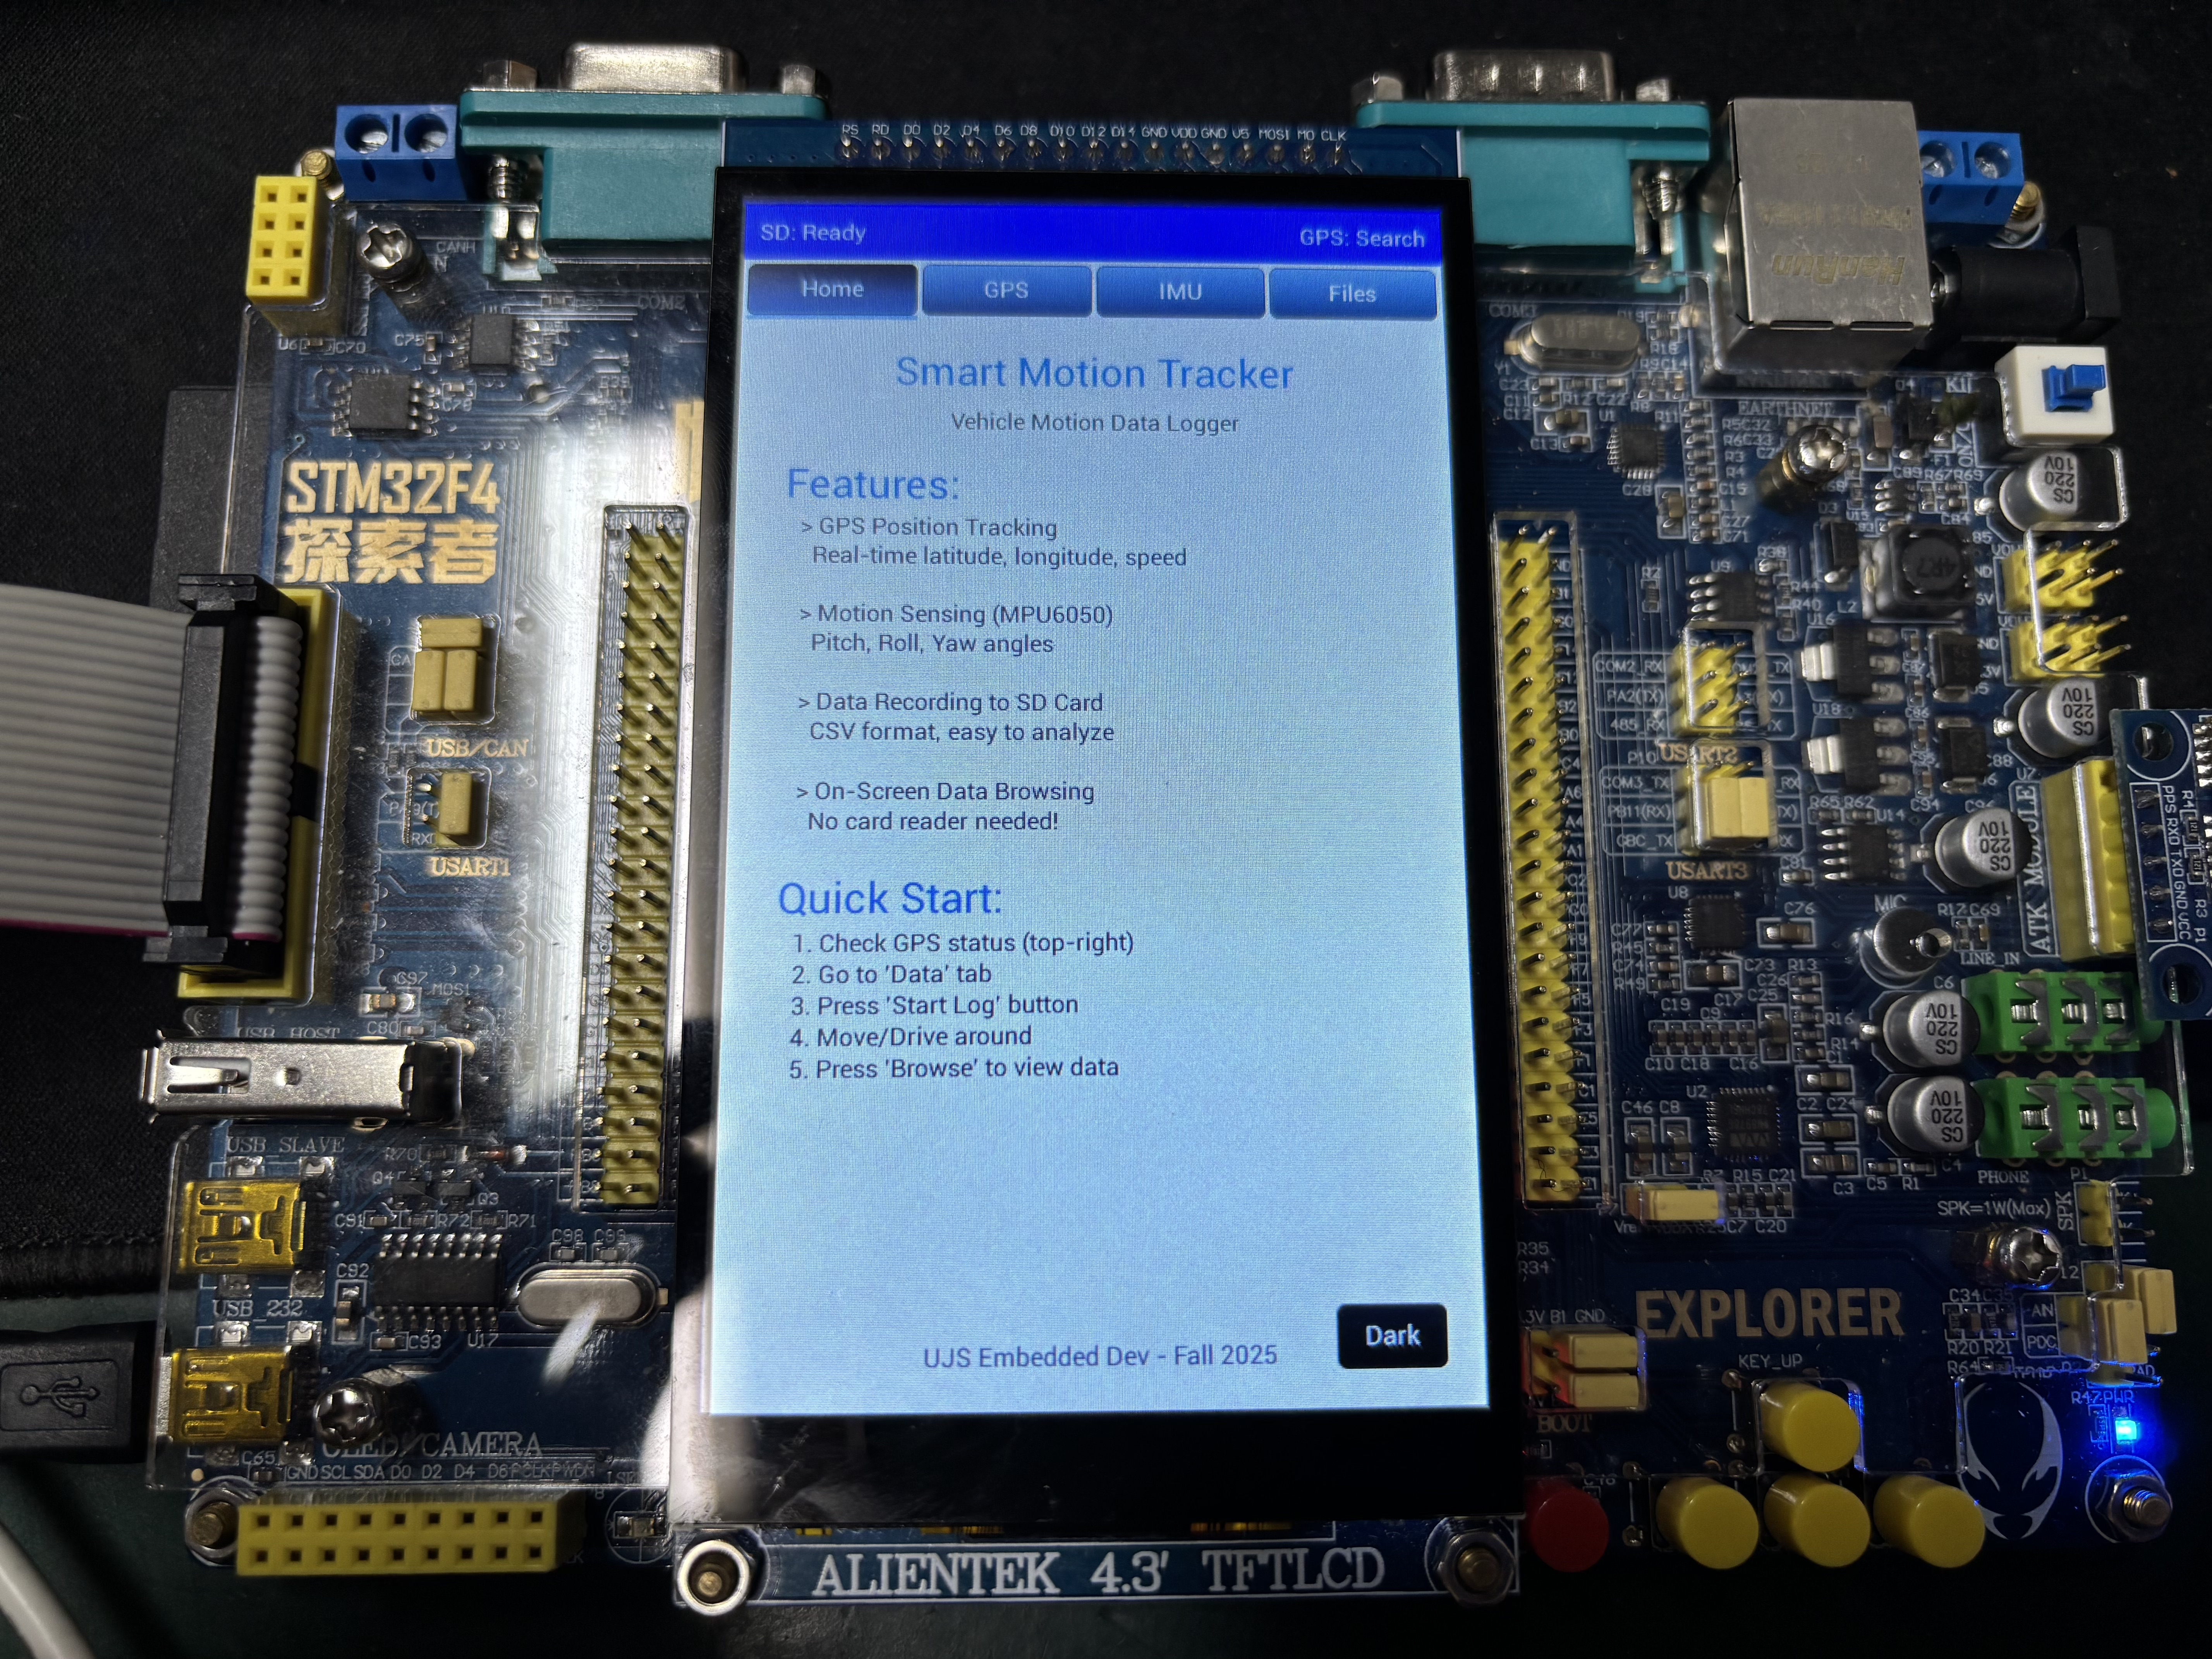
\includegraphics[width=0.9\textwidth]{images/Home界面.png}
    \end{center}
    \footnotesize
    \textit{LVGL 5.3 | 深色模式支持 | 触摸交互}
    \end{columns}
\end{frame}

%% 第三部分：系统演示
\section{系统演示}

\begin{frame}{LCD显示效果}
    \begin{columns}
    \column{0.33\textwidth}
    \begin{center}
    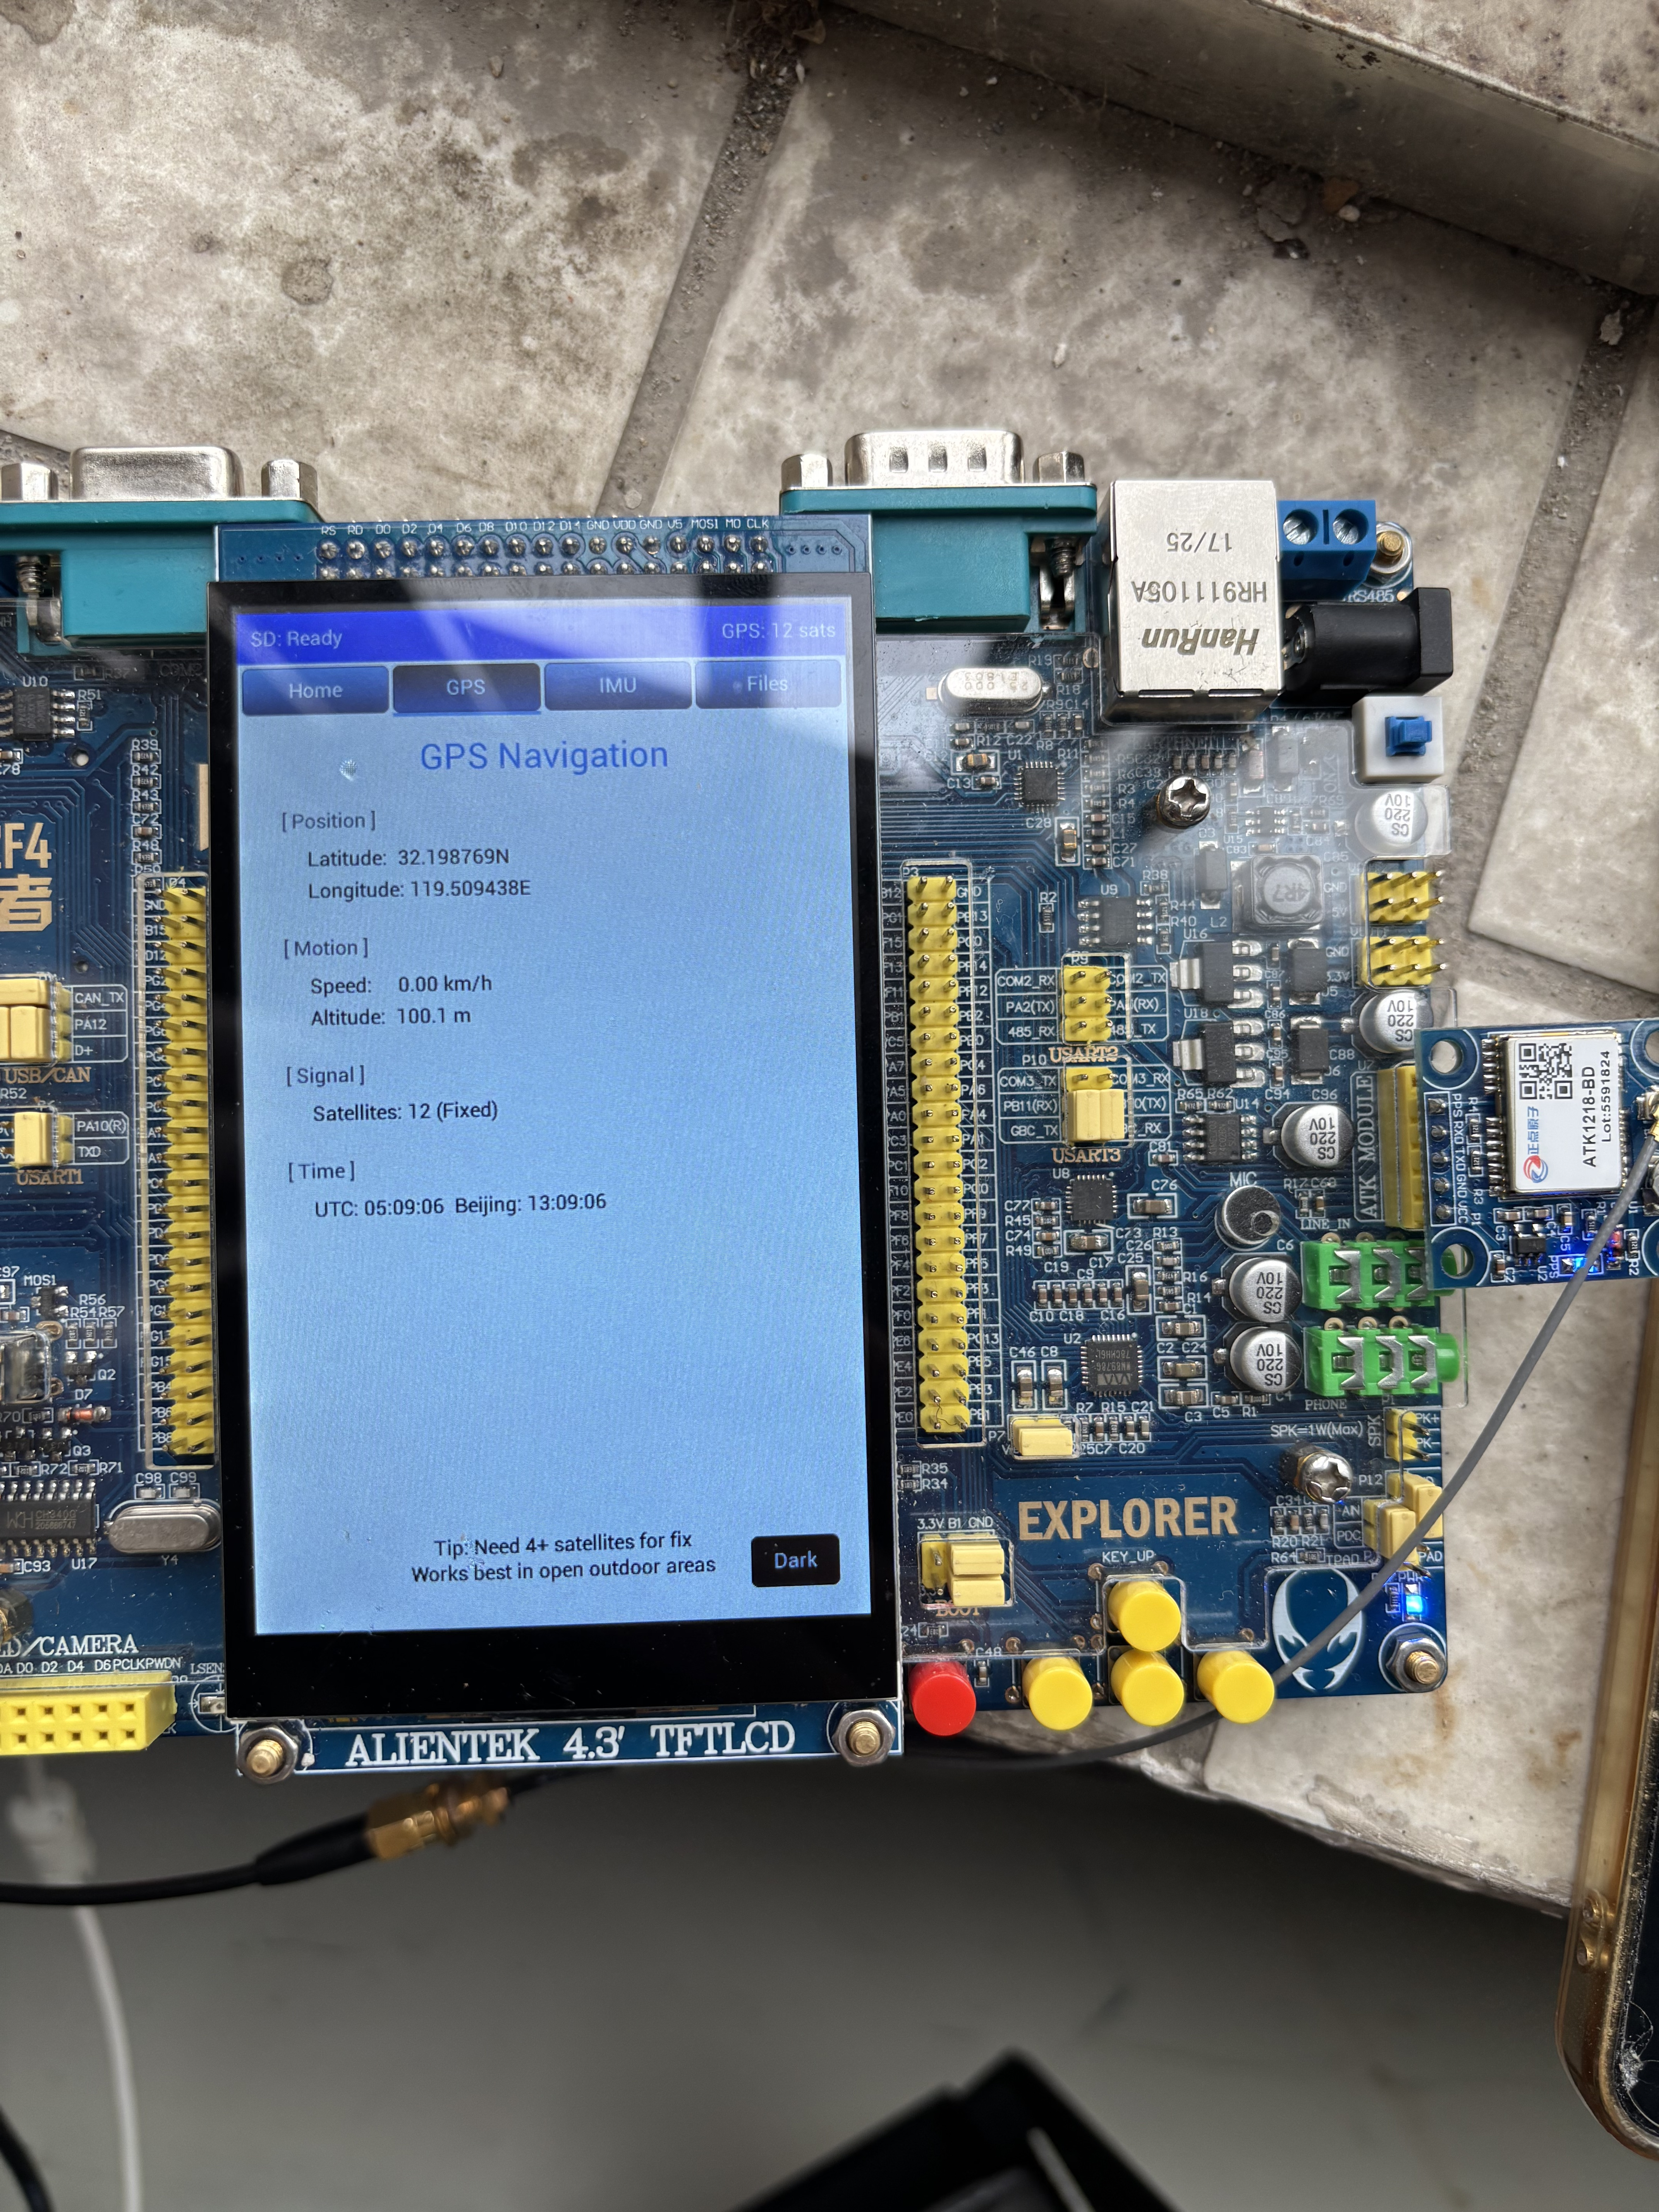
\includegraphics[height=0.55\textheight]{images/GPS页面.png}\\
    \footnotesize GPS页面\\
    {\tiny 实时经纬度、速度、海拔、卫星数}
    \end{center}

    \column{0.33\textwidth}
    \begin{center}
    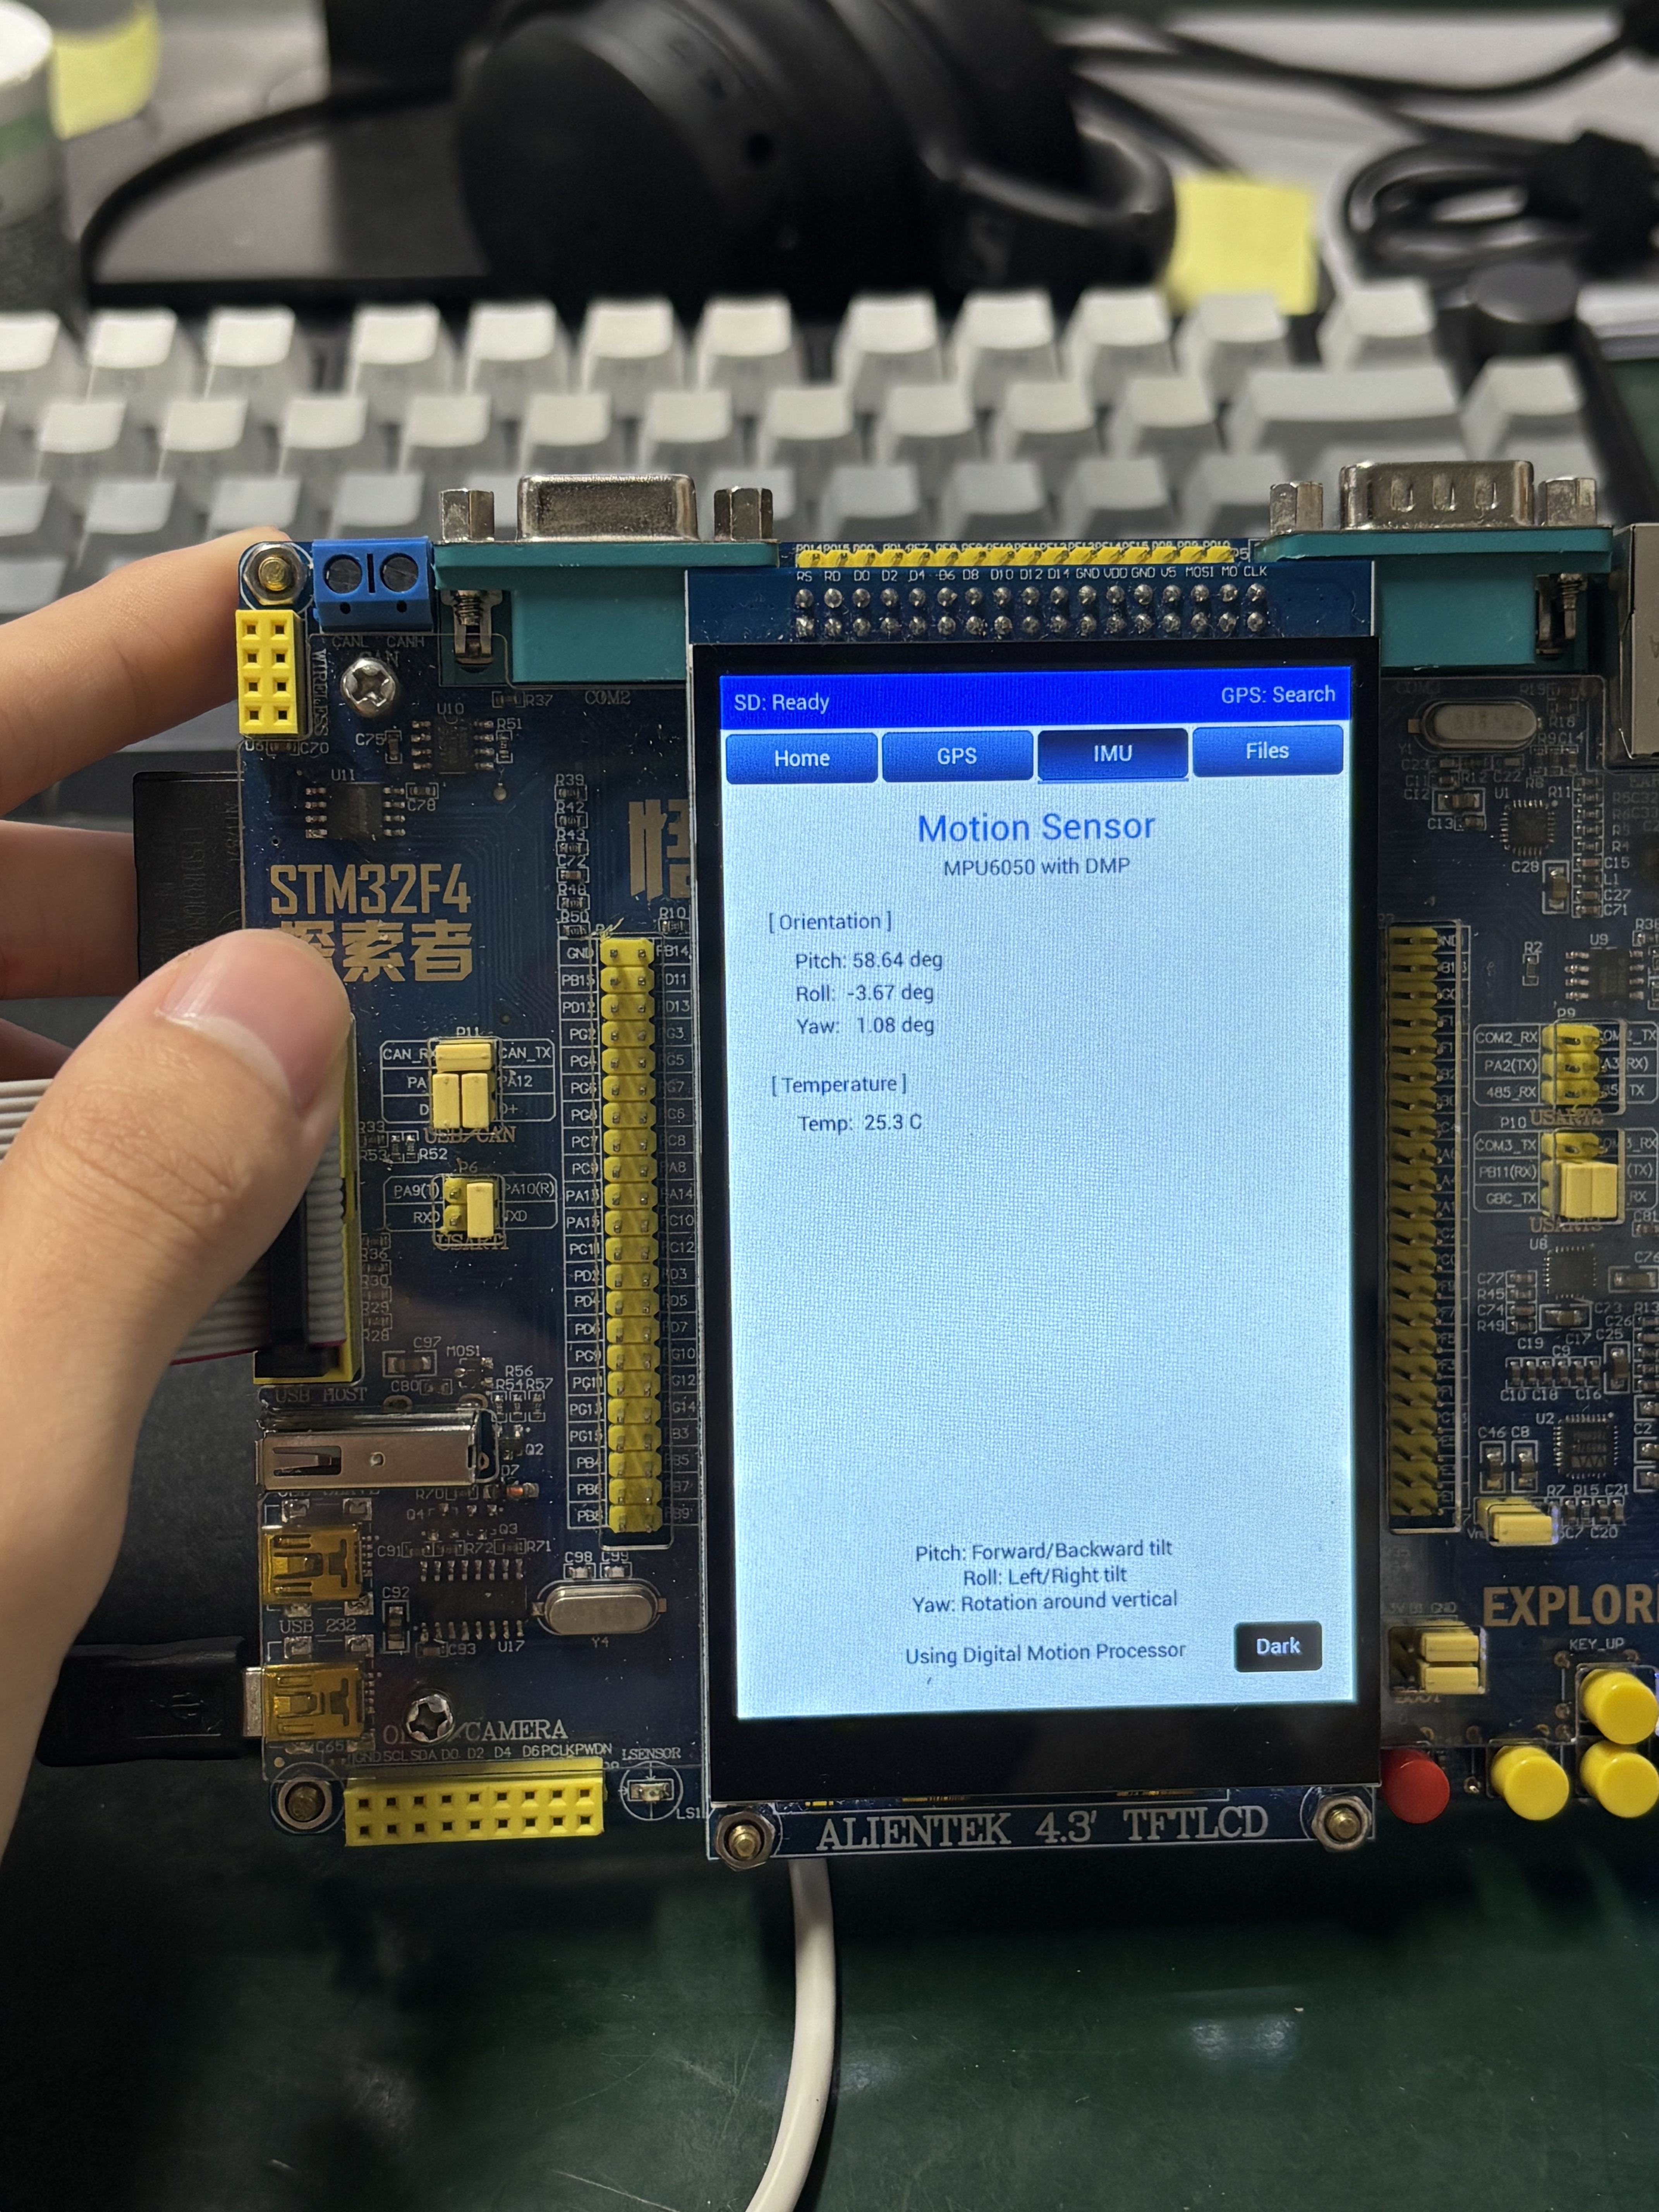
\includegraphics[height=0.55\textheight]{images/IMU界面.png}\\
    \footnotesize IMU页面\\
    {\tiny Pitch/Roll/Yaw三轴姿态角}
    \end{center}

    \column{0.33\textwidth}
    \begin{center}
    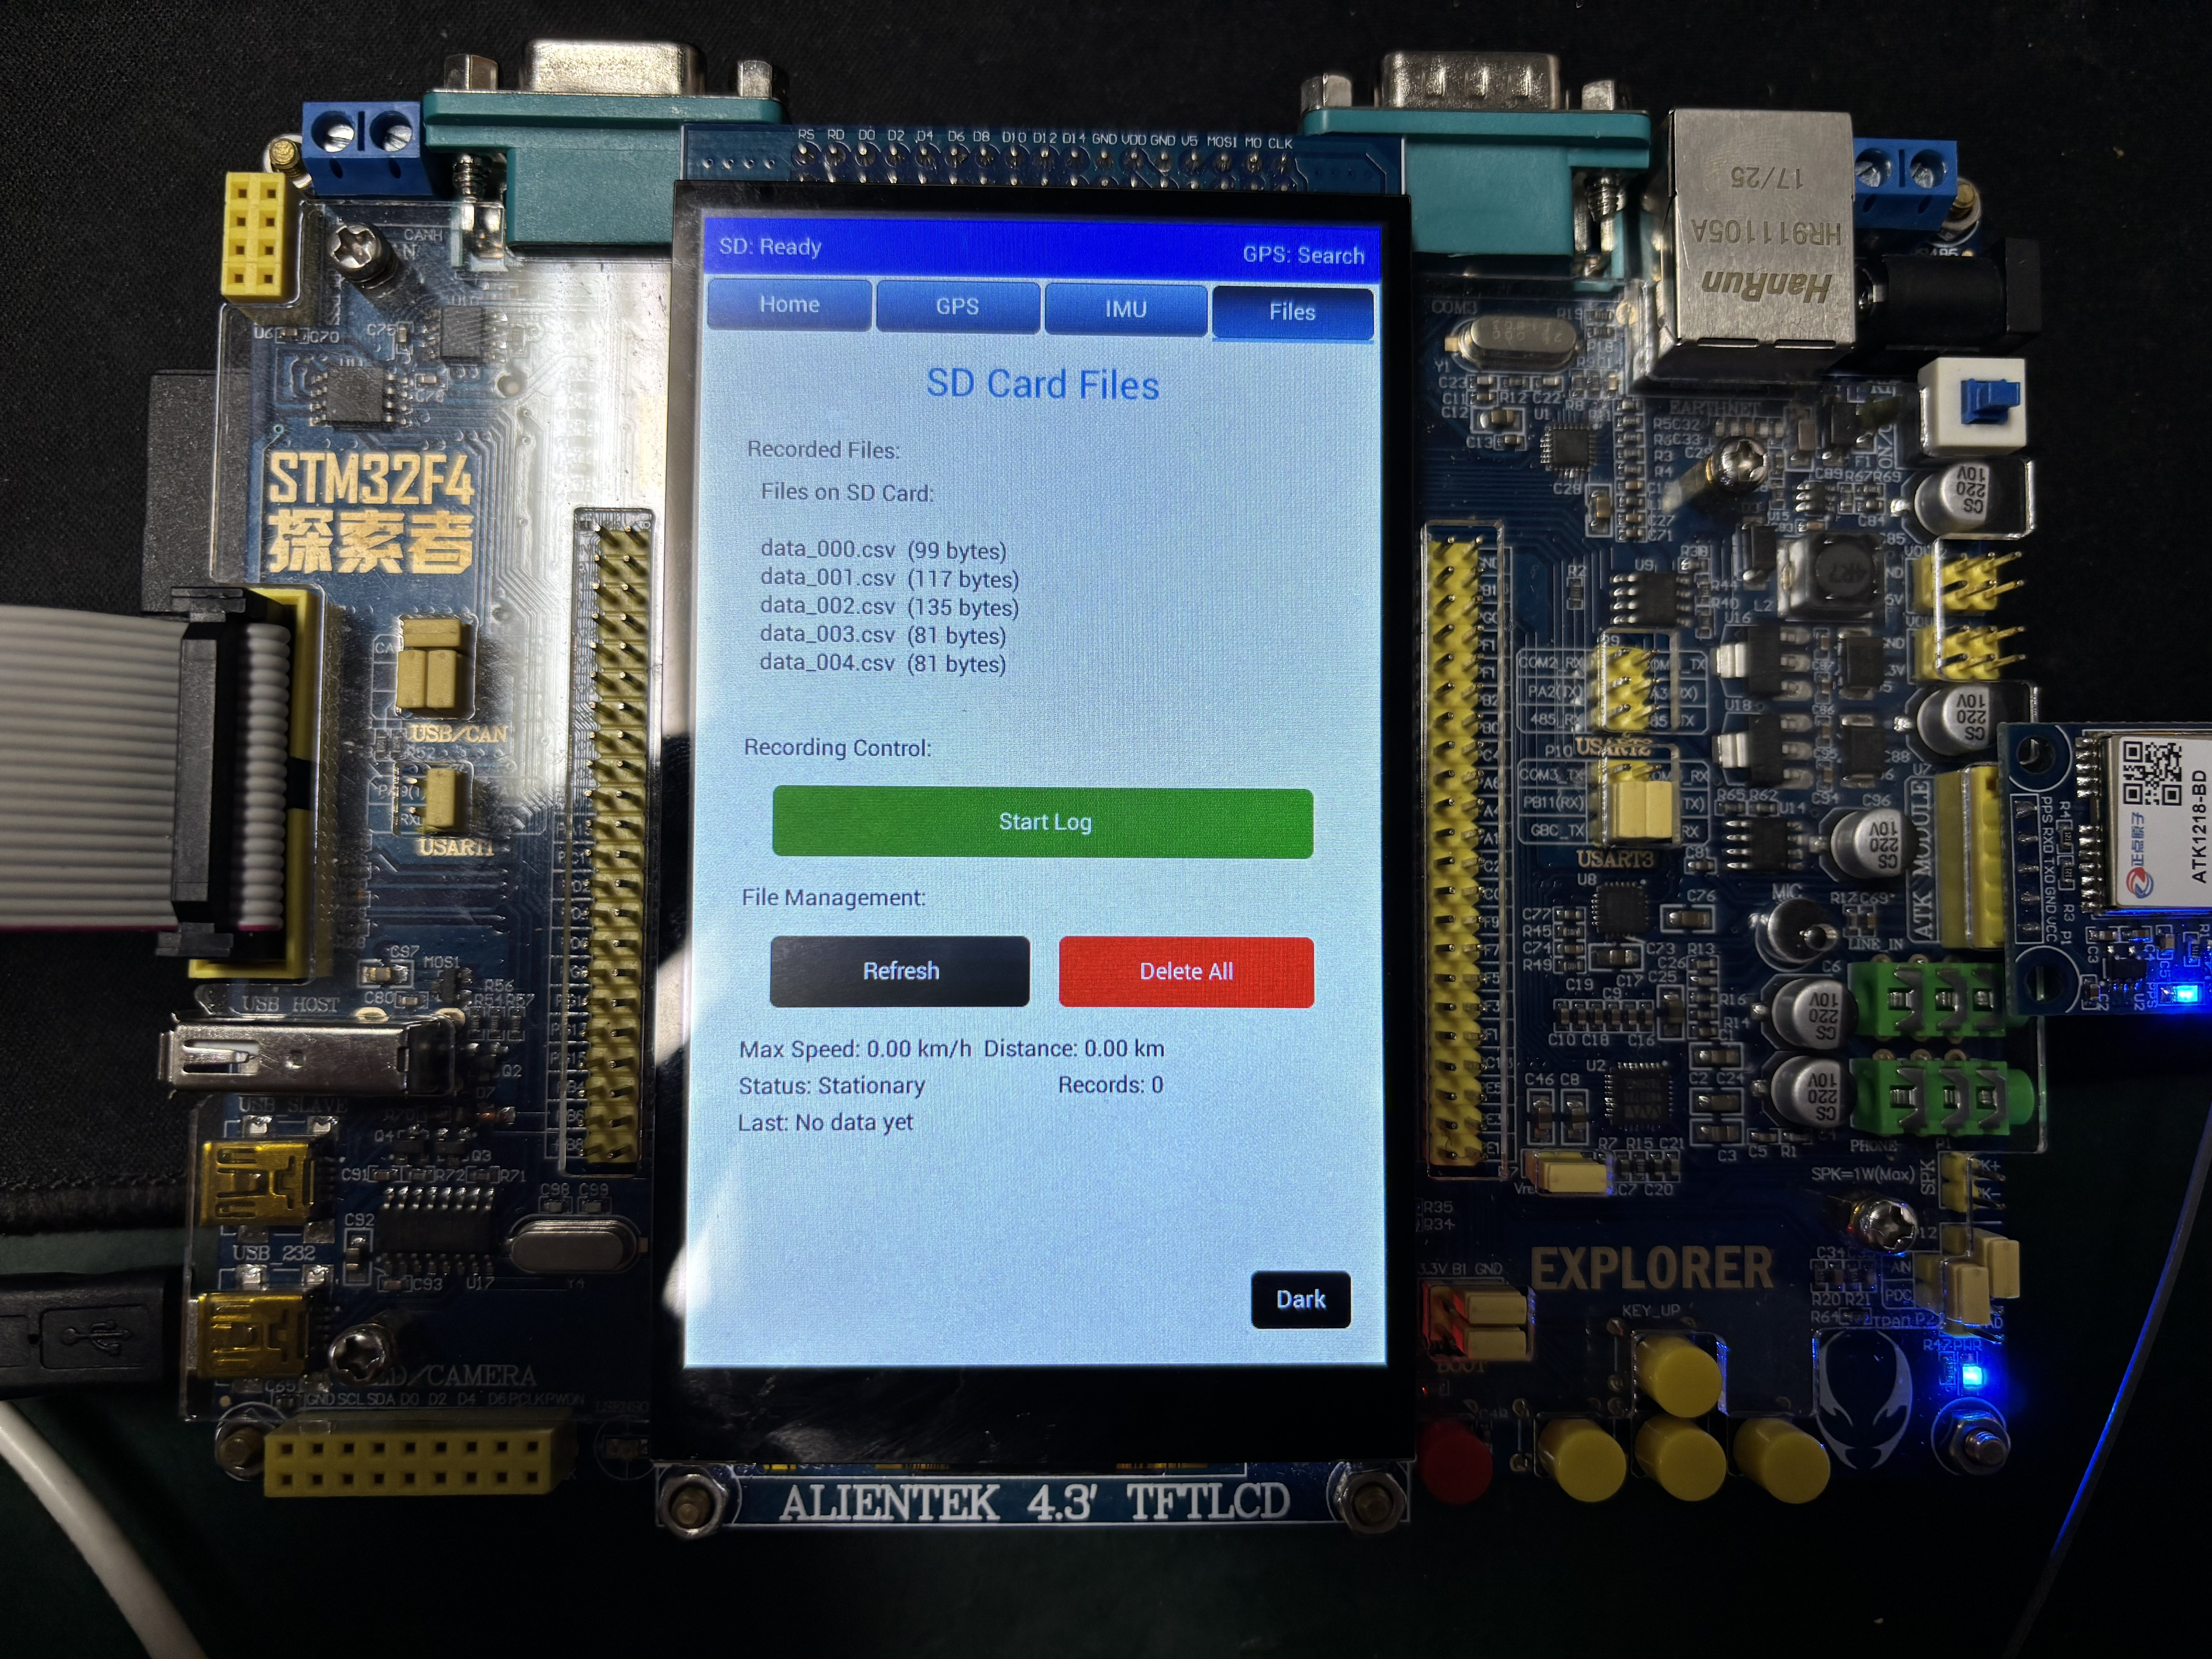
\includegraphics[height=0.55\textheight]{images/files界面.png}\\
    \footnotesize Files页面\\
    {\tiny data\_000.csv \textasciitilde \ data\_004.csv}
    \end{center}
    \end{columns}

    \begin{center}
    {\color{blue}演示视频：完整开机与四页面触摸交互}
    \end{center}
\end{frame}

\begin{frame}{深色模式支持}
    \begin{columns}
    \column{0.5\textwidth}
    \begin{center}
    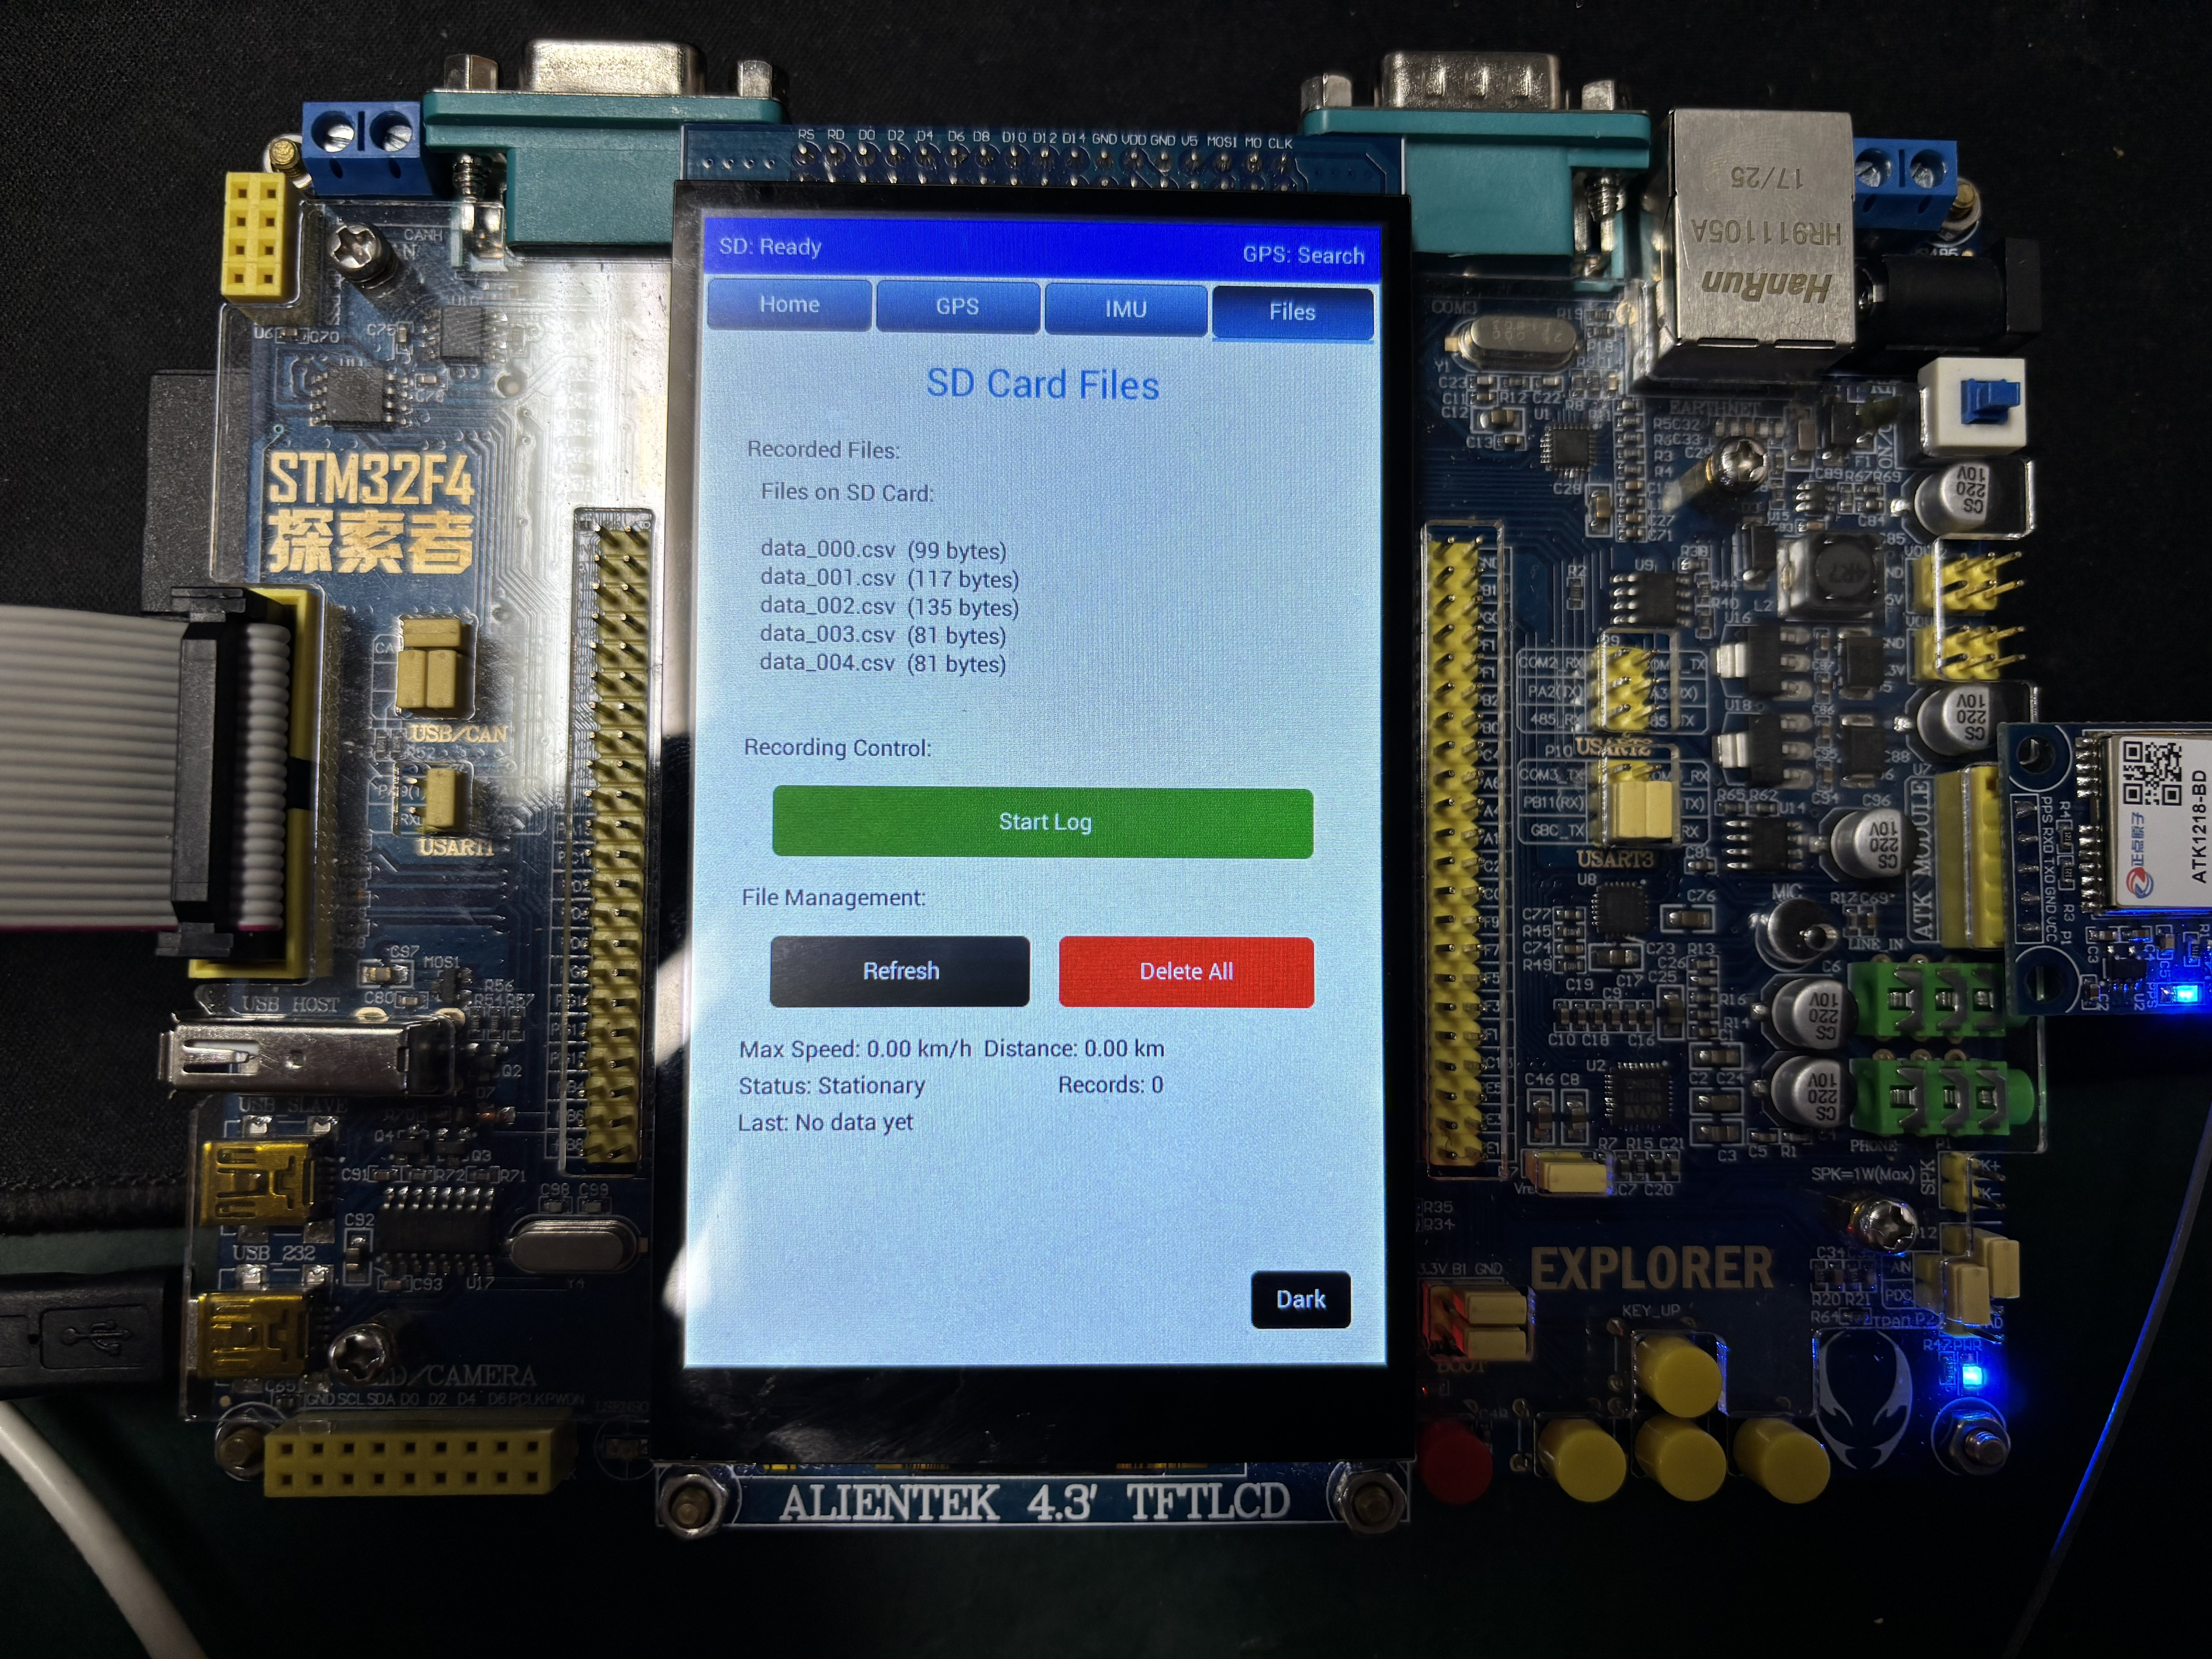
\includegraphics[width=0.9\textwidth]{images/files界面.png}\\
    \footnotesize 浅色模式（默认）
    \end{center}

    \column{0.5\textwidth}
    \begin{center}
    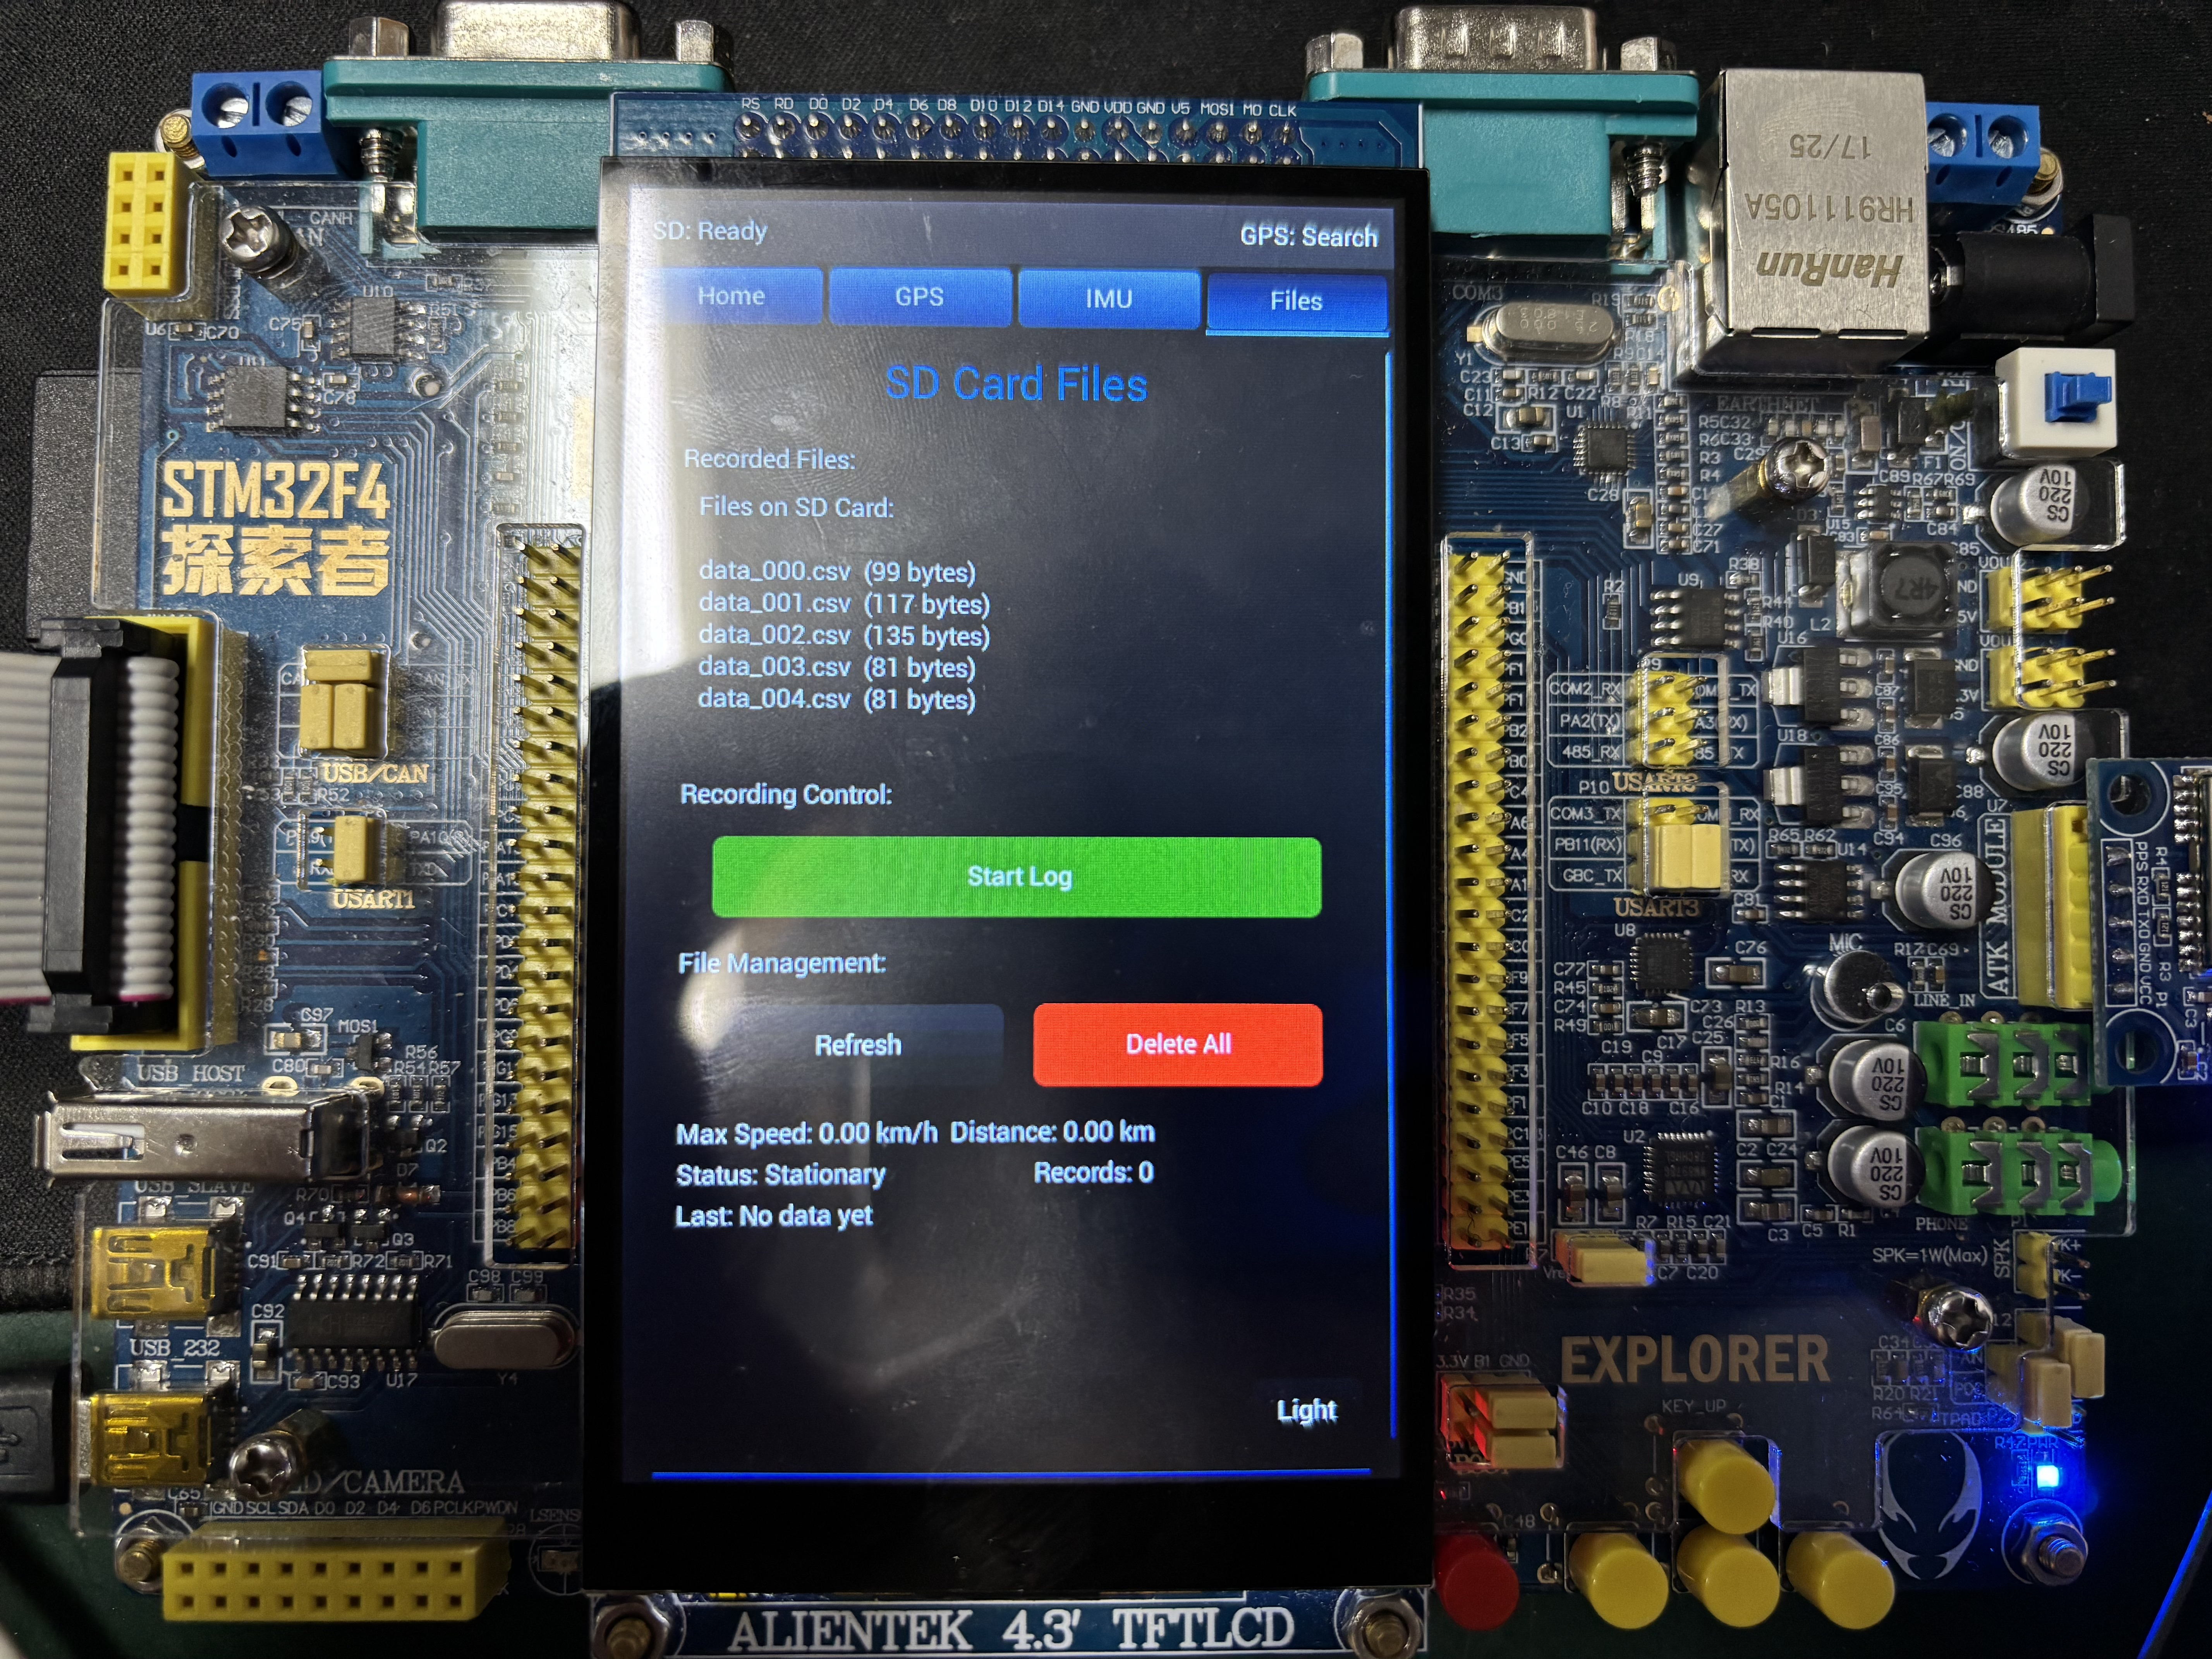
\includegraphics[width=0.9\textwidth]{images/lvgl深色模式.png}\\
    \footnotesize 深色模式
    \end{center}
    \end{columns}

    \vspace{0.5cm}
    \begin{center}
    \textbf{一键切换 | 护眼设计 | 夜间友好}
    \end{center}
\end{frame}

%% 第四部分：Web可视化
\section{Web可视化系统}

\begin{frame}{Web端轨迹分析}
    \begin{columns}
    \column{0.45\textwidth}
    \textbf{核心功能：}
    \begin{itemize}
        \item Leaflet.js地图引擎
        \item 轨迹热力图（速度着色）
        \item Chart.js速度曲线
        \item 7项统计指标
        \item 动画回放功能
        \item 报告导出（TXT）
    \end{itemize}

    \vspace{0.3cm}
    \textbf{技术栈：}
    \begin{itemize}
        \item 前端：HTML5 + JavaScript
        \item 地图：Leaflet.js + OpenStreetMap
        \item 图表：Chart.js
        \item 深色模式 + 响应式布局
    \end{itemize}

    \column{0.55\textwidth}
    \begin{center}
    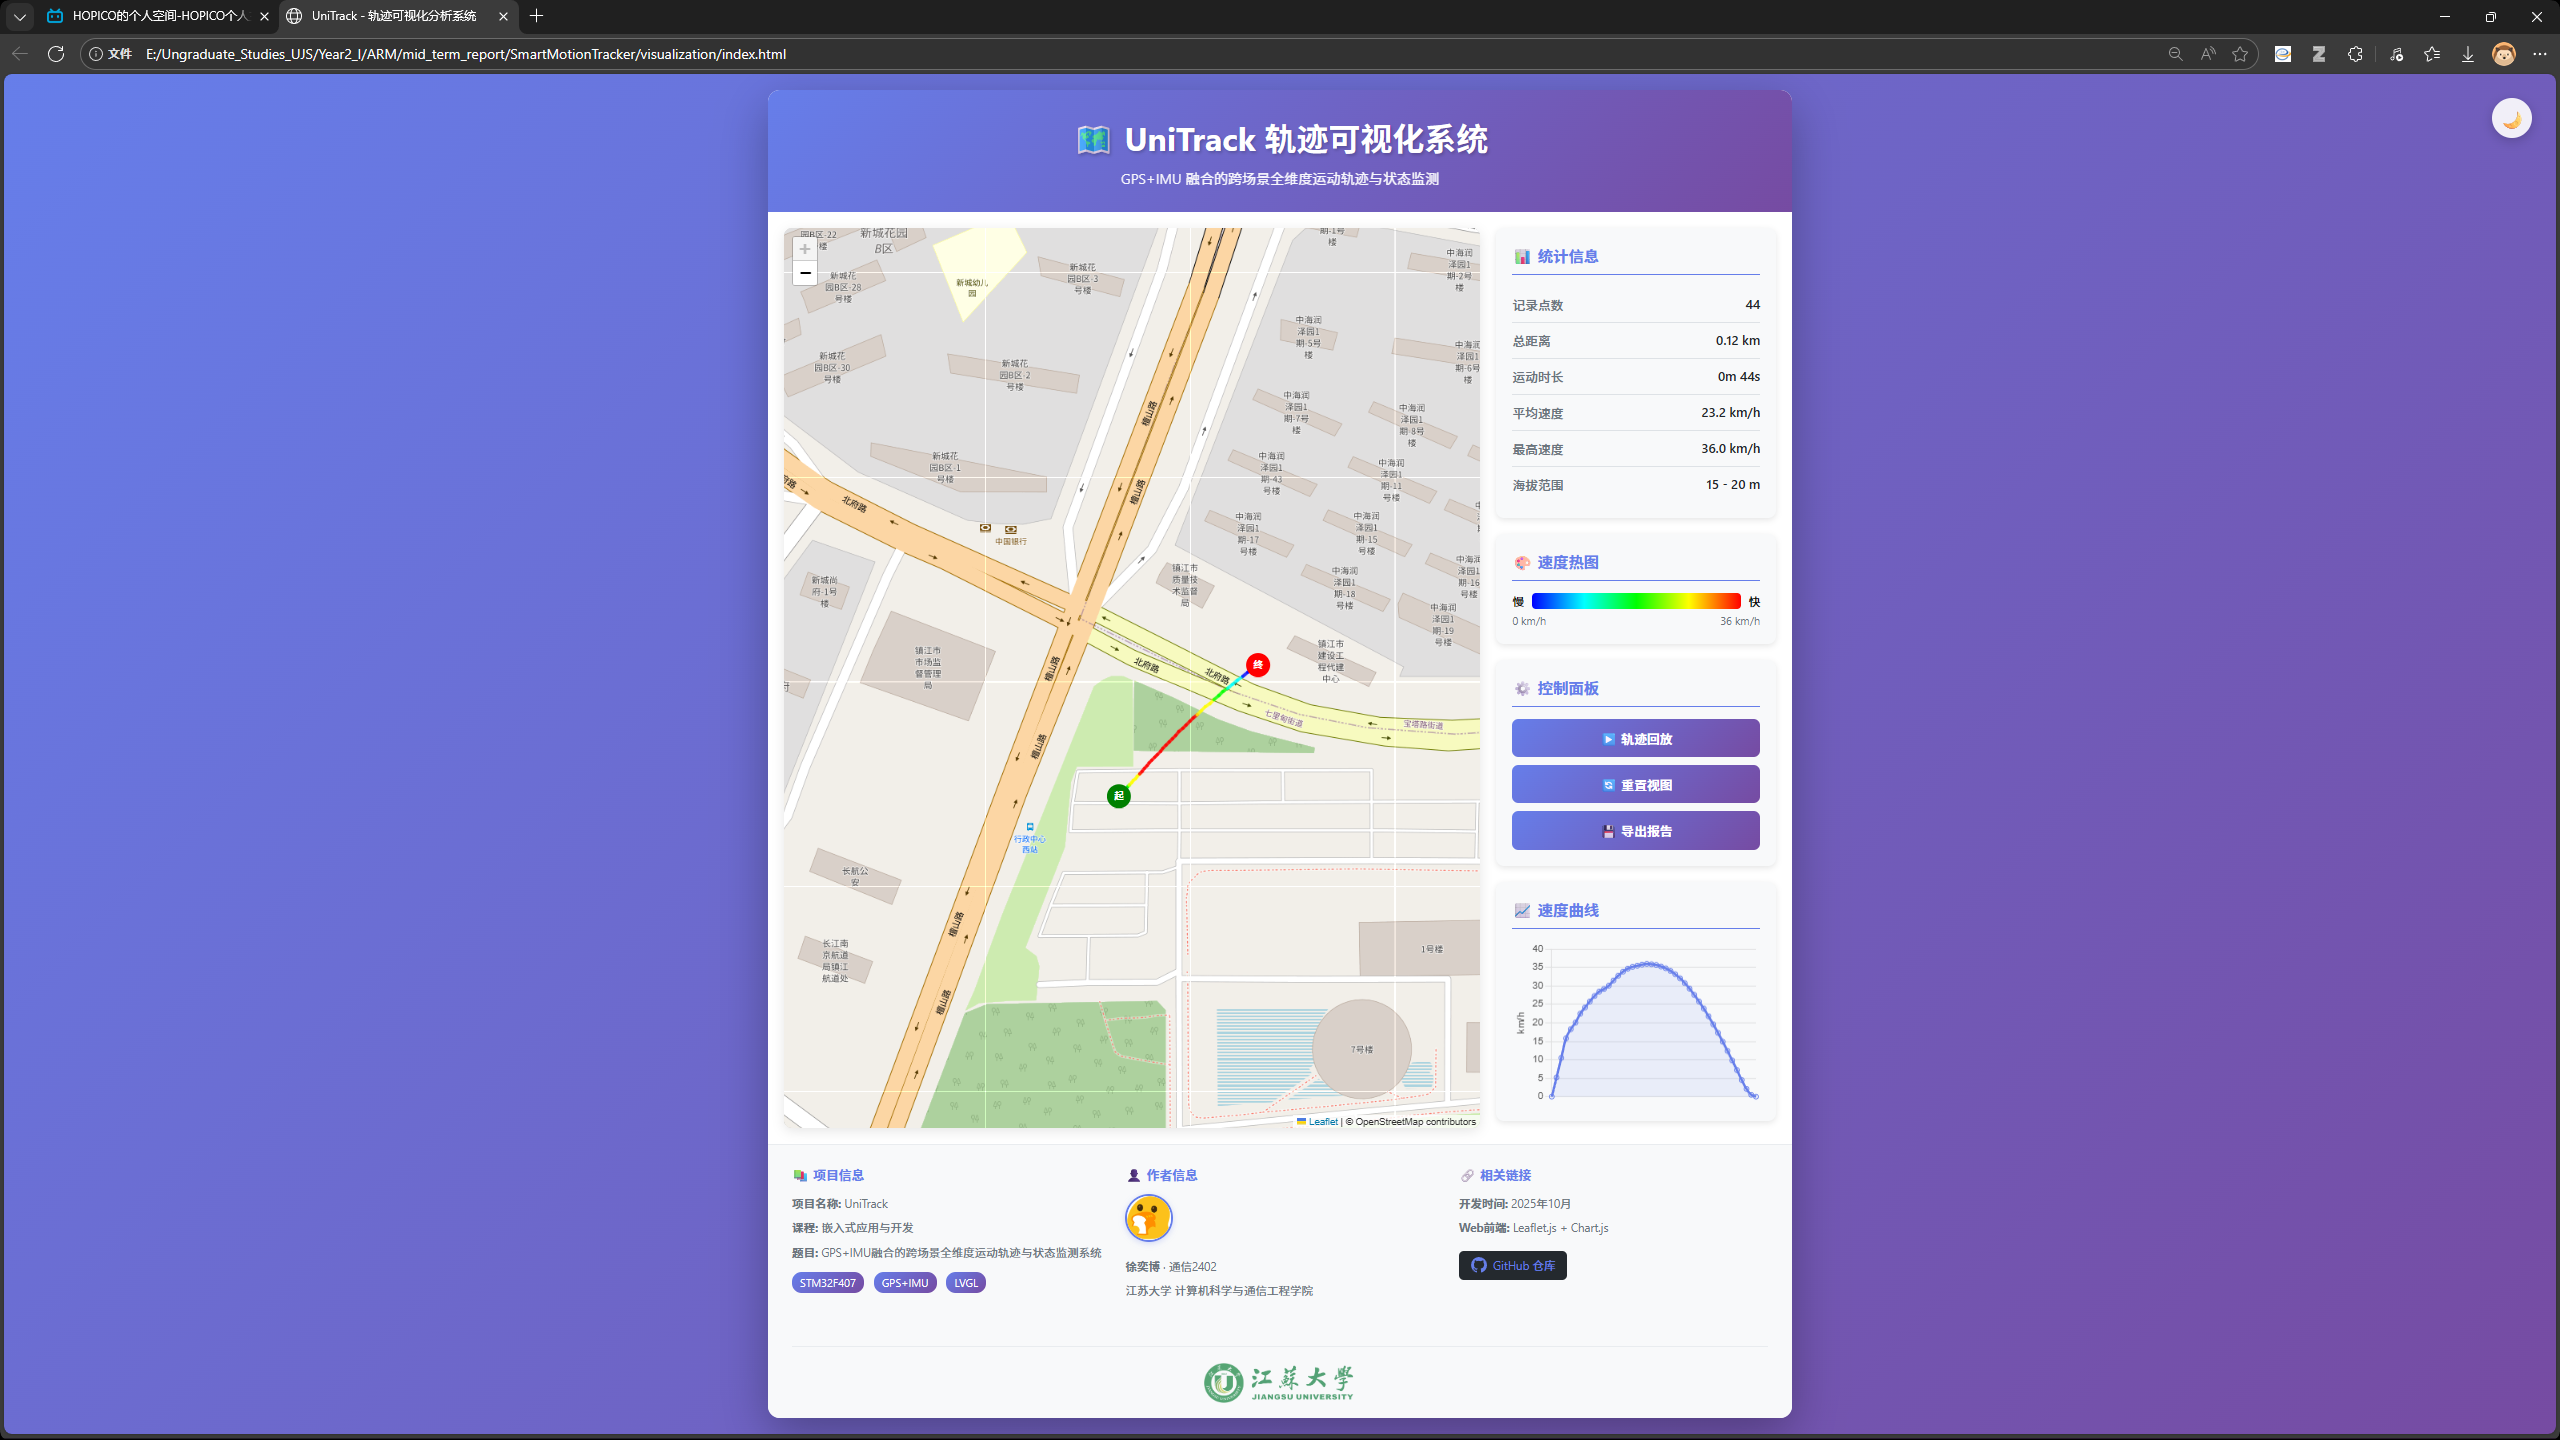
\includegraphics[width=\textwidth]{images/可视化网页截图.png}
    \end{center}
    \footnotesize
    \textit{支持CSV拖拽上传 | 实时数据分析}
    \end{columns}
\end{frame}

\begin{frame}{Web深色模式}
    \begin{center}
    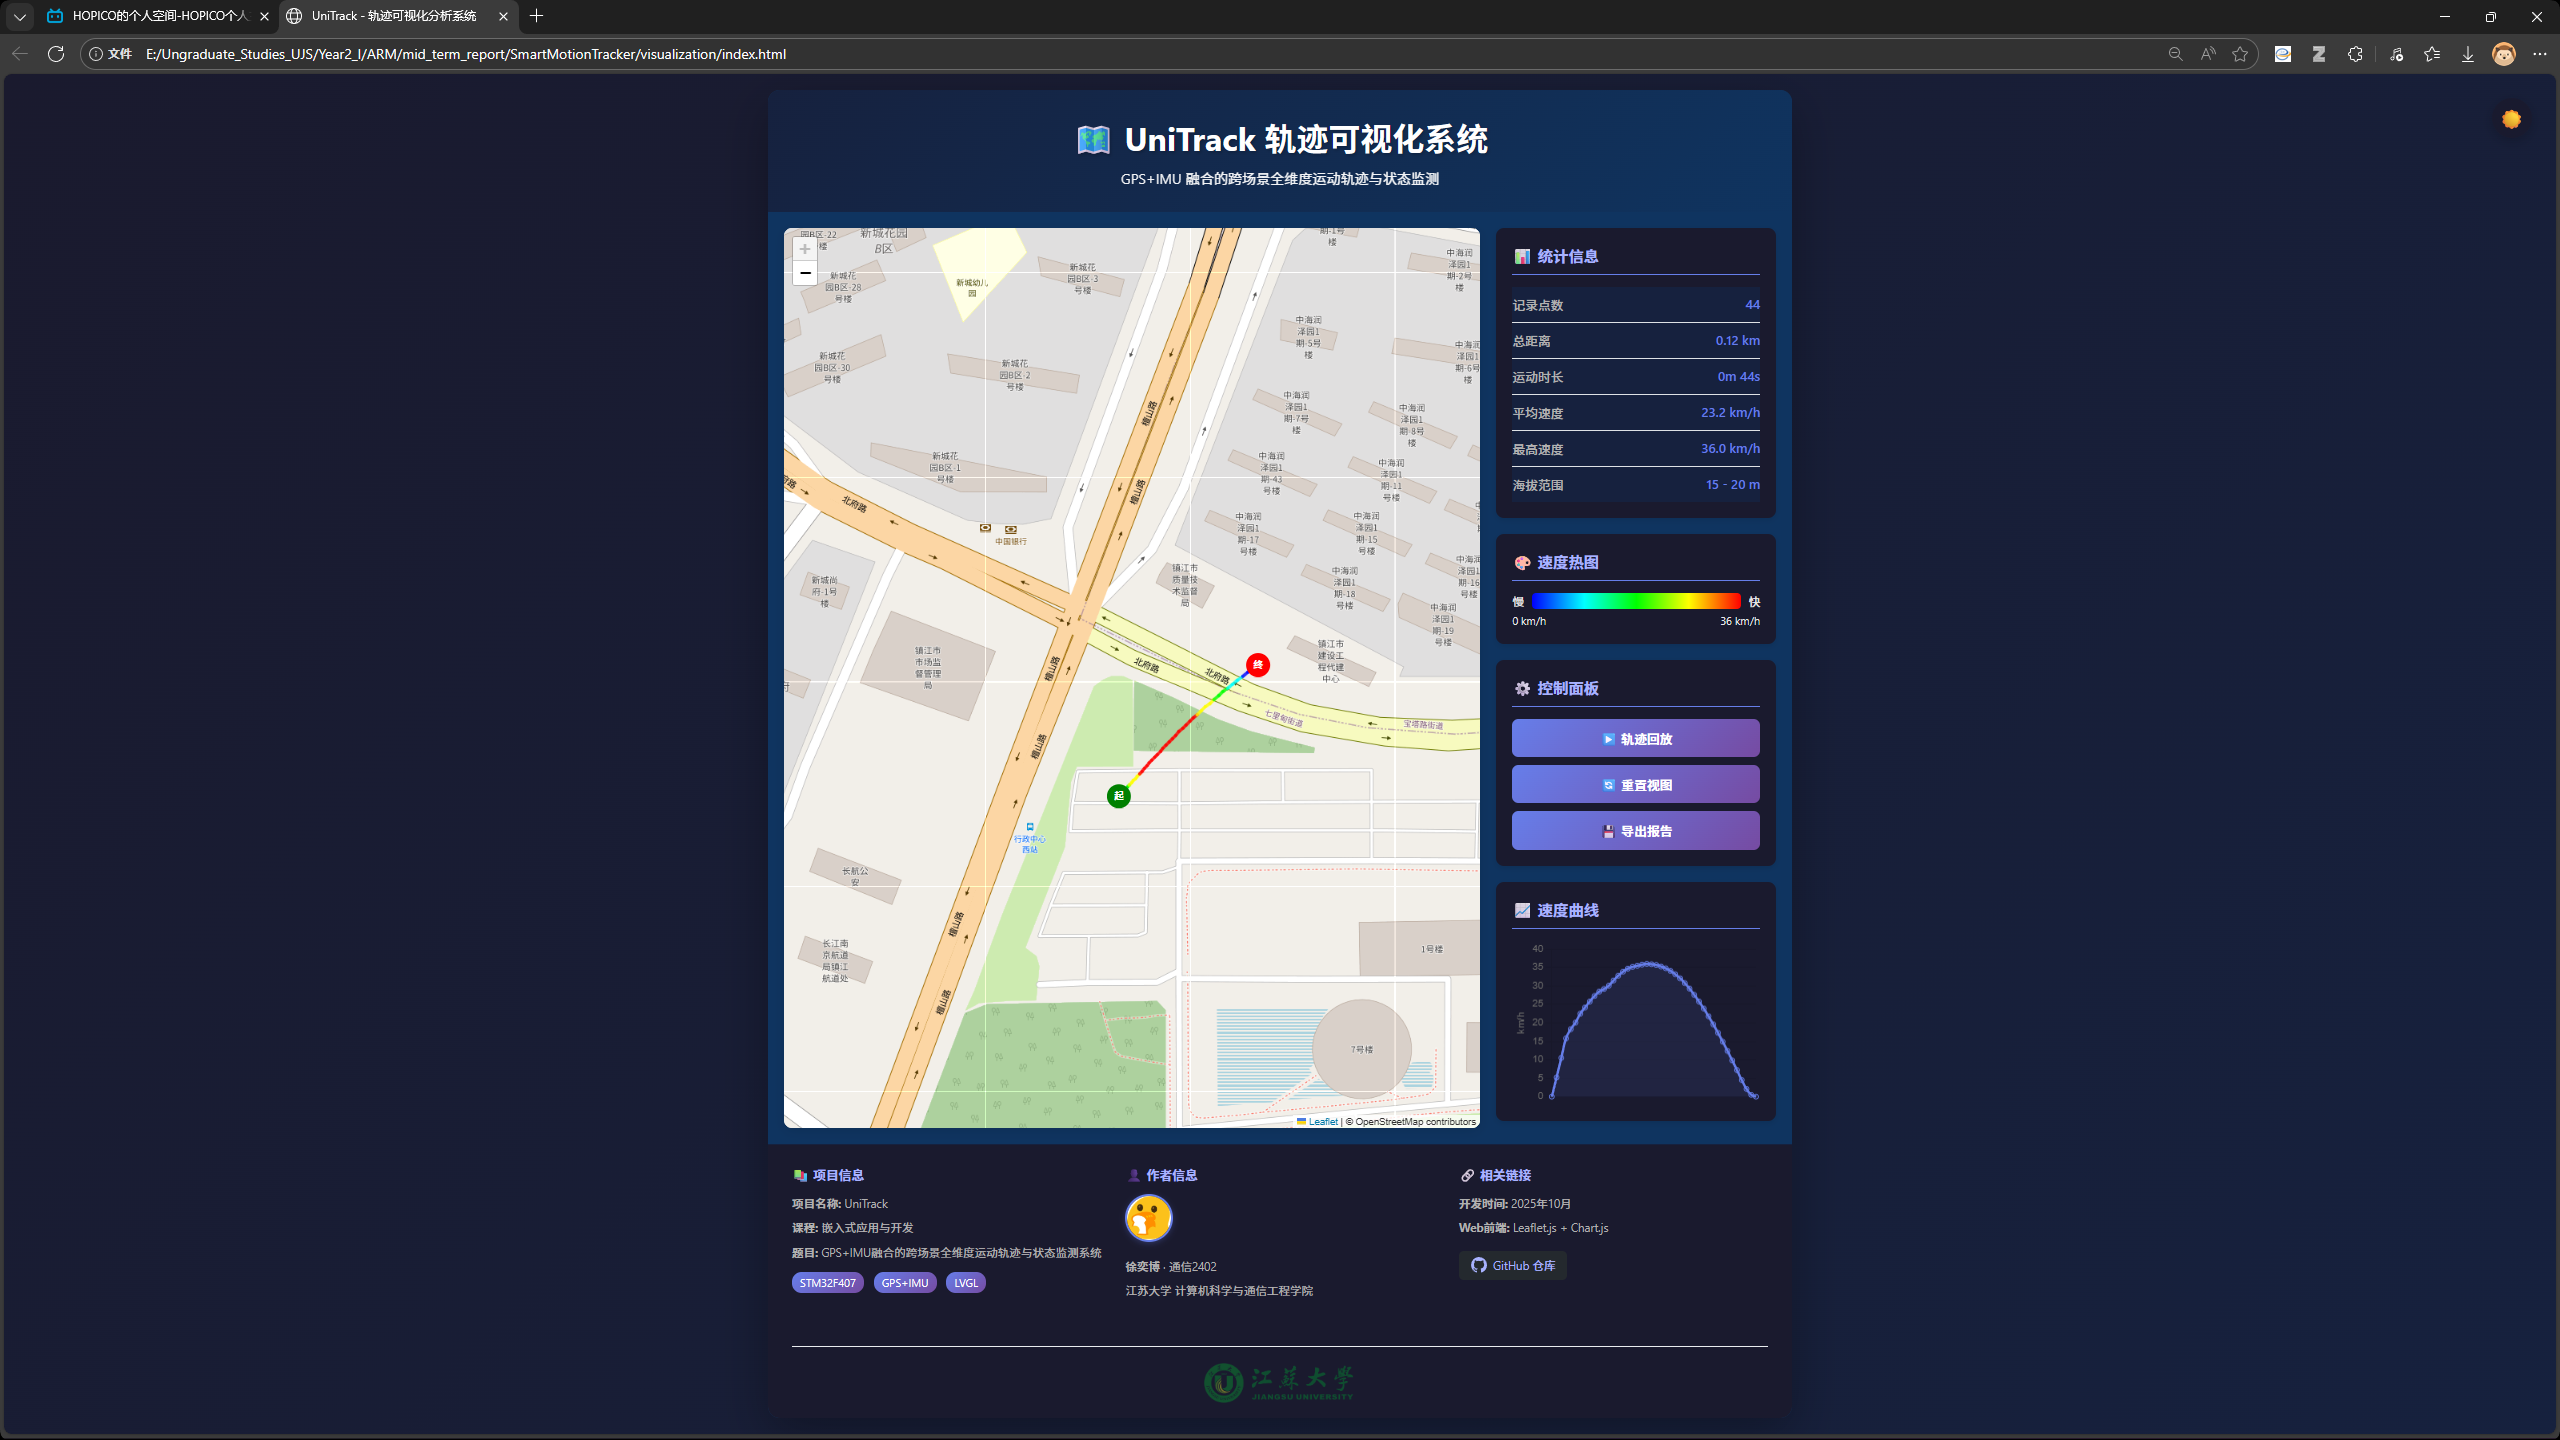
\includegraphics[height=0.7\textheight]{images/可视化网页深色模式演示截图.png}
    \end{center}
\end{frame}

%% 第五部分：开发总结
\section{开发总结}

\begin{frame}{开发过程中的挑战}
    \begin{block}{1. GPS模块调试（{\color{red}耗时最长}）}
    \begin{itemize}
        \item {\color{red}问题：}跳线帽连接错误 + 模块型号识别错误
        \item {\color{green!60!black}解决：}查阅ATK-MO1218手册，正确连接P2端子，切换例程
    \end{itemize}
    \end{block}
    \vspace{-0.2cm}
    \begin{block}{2. 内存资源优化（{\color{red}61条L6406E错误}）}
    \begin{itemize}
        \item {\color{red}问题：}FATFS + LVGL内存需求超出RAM容量
        \item {\color{green!60!black}解决：}malloc从100KB降至40KB，正确配置IRAM1=128KB
    \end{itemize}
    \end{block}
    \vspace{-0.2cm}
    \begin{block}{3. 外设库文件缺失（{\color{red}L6218E错误}）}
    \begin{itemize}
        \item {\color{red}问题：}DMA、SDIO、SPI驱动文件未添加
        \item {\color{green!60!black}解决：}补充STM32F4xx标准外设库
    \end{itemize}
    \end{block}
\end{frame}

\begin{frame}{系统性能指标}
\begin{table}
\centering
\begin{tabular}{|c|c|c|}
\hline
\textbf{指标} & \textbf{参数值} & \textbf{说明} \\
\hline
GPS定位精度 & 2.5m CEP & 开阔环境下 \\
\hline
IMU采样率 & 100Hz & DMP输出频率 \\
\hline
数据记录频率 & 10Hz & 可配置 \\
\hline
UI刷新率 & 100Hz & LVGL任务处理 \\
\hline
存储容量 & 8GB & 支持>2000小时 \\
\hline
功耗 & 约1.2W & 工作状态 \\
\hline
\end{tabular}
\end{table}
\end{frame}

\begin{frame}{项目创新点}
\begin{enumerate}
    \item \textbf{多源数据融合：}GPS + IMU协同，提供全维度运动信息
    \item \textbf{全栈设计：}嵌入式底层→Web前端完整数据链路
    \item \textbf{双端可视化：}LCD实时显示 + Web离线深度分析
    \item \textbf{高可靠性：}文件索引管理、断电保护、数据同步
    \item \textbf{用户体验：}深色模式、响应式布局、动画回放
    \item \textbf{开源共享：}完整代码开源于GitHub
\end{enumerate}

\vspace{0.5cm}
\begin{center}
\url{https://github.com/XCMB-haochi/2025-ARM-MidTerm-HW-SmartMotionTracker}
\end{center}
\end{frame}

%% 第六部分：致谢
\section*{}

\begin{frame}
    \vfill
    \centering
    \Huge \textbf{感谢各位的聆听！}

    \vspace{1cm}

    \Large \textbf{欢迎提问与指导}
    \vfill
\end{frame}

\end{document}
